% ============================================================================
% Agentic Programming: Using AI Agents for Research
% Duration: ~4 hours (two 90-min blocks with breaks + exercises)
% ============================================================================

\documentclass[aspectratio=169,10pt]{beamer}

% ---------- Theme and colors ----------
\usecolortheme{dove}
\setbeamertemplate{navigation symbols}{}
\setbeamertemplate{footline}{%
  \hfill\usebeamerfont{page number in head/foot}%
  \usebeamercolor[fg]{normal text}%
  \insertframenumber\,/\,\inserttotalframenumber\kern1em\vskip4pt}
\setbeamerfont{frametitle}{size=\huge}

% ---------- Packages ----------
\usepackage[utf8]{inputenc}
\usepackage[T1]{fontenc}
\usepackage{amsmath,amssymb,amsfonts}
\usepackage{bm}
\usepackage{graphicx}
\usepackage{tikz}
\usetikzlibrary{shapes,arrows.meta,positioning,calc,fit,backgrounds,
                 patterns,decorations.pathreplacing,shadows.blur}
\usepackage{pgfplots}
\pgfplotsset{compat=1.18}
\usepackage{booktabs}
\usepackage{hyperref}
\usepackage{multicol}
\usepackage{xcolor}
\usepackage{algorithm}
\usepackage{algorithmic}
\usepackage{listings}
\usepackage{pifont}
\usepackage{colortbl}

% ---------- Listings ----------
\lstset{
    language=Python,
    basicstyle=\small\ttfamily,
    keywordstyle=\color{uzhblue}\bfseries,
    commentstyle=\color{uzhgreydark}\itshape,
    stringstyle=\color{darkgreen},
    showstringspaces=false,
    breaklines=true,
    frame=none,
    xleftmargin=0pt,
    aboveskip=4pt,
    belowskip=4pt,
    escapeinside={(*@}{@*)},
}
\lstdefinestyle{bash}{
    language=bash,
    basicstyle=\small\ttfamily,
    keywordstyle=\color{uzhblue}\bfseries,
    commentstyle=\color{uzhgreydark}\itshape,
    stringstyle=\color{darkgreen},
    showstringspaces=false,
    breaklines=true, frame=none,
    xleftmargin=0pt, aboveskip=4pt, belowskip=4pt,
    morekeywords={claude,git,uv,npm,pip,cd,mkdir,ssh,squeue,sbatch},
}
\lstdefinestyle{prompt}{
    basicstyle=\small\ttfamily,
    breaklines=true, frame=none,
    xleftmargin=6pt, aboveskip=4pt, belowskip=4pt,
    literate={>}{{\textcolor{harvardcrimson}{>}}}1,
}

% ---------- Custom colors ----------
\definecolor{uzhblue}{rgb}{0,0,0.5}
\definecolor{uzhgreylight}{RGB}{236,238,241}
\definecolor{uzhgreydark}{RGB}{81,86,94}
\definecolor{harvardcrimson}{RGB}{153,0,0}
\definecolor{unil@blue}{RGB}{0,140,204}
\definecolor{unil@black}{RGB}{35,31,32}
\definecolor{darkgreen}{RGB}{0,100,0}
\definecolor{darkred}{RGB}{139,0,0}
\definecolor{softblue}{RGB}{70,130,180}
\definecolor{softorange}{RGB}{230,159,0}
\definecolor{softgreen}{RGB}{0,158,115}
\definecolor{level0}{RGB}{200,200,200}
\definecolor{level1}{RGB}{180,200,220}
\definecolor{level2}{RGB}{140,180,220}
\definecolor{level3}{RGB}{100,160,220}
\definecolor{level4}{RGB}{60,130,200}
\definecolor{level5}{RGB}{30,90,160}

% ---------- Set beamer colors ----------
\setbeamercolor{frametitle}{bg=uzhgreylight, fg=uzhblue}
\setbeamercolor{title}{fg=uzhblue}
\setbeamercolor{structure}{fg=uzhblue}
\setbeamercolor{block title}{bg=unil@blue, fg=white}
\setbeamercolor{block body}{bg=uzhgreylight}
\setbeamercolor{block title alerted}{bg=darkred,fg=white}
\setbeamercolor{block body alerted}{bg=red!5}
\setbeamercolor{block title example}{bg=darkgreen,fg=white}
\setbeamercolor{block body example}{bg=green!5}
\setbeamercolor{item}{fg=unil@black}
\setbeamercolor{normal text}{fg=unil@black}

% ---------- Commands ----------
\newcommand{\emphc}[1]{\textcolor{harvardcrimson}{#1}}
\hypersetup{colorlinks,linkcolor=harvardcrimson,urlcolor=harvardcrimson}
\newcommand{\R}{\mathbb{R}}
\newcommand{\livedemo}{%
  \tikz[baseline=(X.base)]{\node[fill=harvardcrimson,text=white,
  rounded corners=2pt,inner sep=3pt,font=\scriptsize\bfseries](X){DEMO};}}
% \selfstudy: marks a transcript that self-study readers can follow without an instructor.
\newcommand{\selfstudy}{%
  \tikz[baseline=(X.base)]{\node[fill=softgreen!80!black,text=white,
  rounded corners=2pt,inner sep=2pt,font=\tiny\bfseries](X){SELF-STUDY};}}
\newcommand{\boristip}[1]{%
  \tikz[baseline=(X.base)]{\node[fill=level4,text=white,
  rounded corners=2pt,inner sep=2pt,font=\tiny\bfseries](X){TIP #1};}}

% ---------- TikZ styles defined globally (avoids #1 issues in beamer) ----------
\tikzset{
    cbox/.style={draw, rounded corners=4pt, minimum height=1.2cm,
                 minimum width=2.6cm, align=center, font=\small,
                 fill=#1, text=white},
    phase/.style={draw, rounded corners=3pt, fill=#1,
                  minimum width=4cm, minimum height=0.7cm,
                  font=\scriptsize, align=center},
    spoke/.style={draw, rounded corners=3pt, fill=#1,
                  minimum width=1.6cm, minimum height=0.55cm,
                  font=\tiny, text=white, align=center},
    fblock/.style={draw, rounded corners=5pt, fill=#1,
                   minimum width=2.6cm, minimum height=0.8cm,
                   font=\small, text=white, align=center},
    pstep/.style={draw, rounded corners=3pt, fill=#1,
                  minimum width=2.6cm, minimum height=0.6cm,
                  font=\scriptsize, align=center},
    pcomp/.style={draw, rounded corners=4pt, fill=#1,
                  minimum width=2cm, minimum height=0.9cm,
                  font=\scriptsize, text=white, align=center},
    pipestep/.style={draw, rounded corners=3pt, fill=#1,
                     minimum width=2.6cm, minimum height=0.55cm,
                     font=\tiny, text=white, align=center},
    rung/.style={draw, rounded corners=2pt, fill=#1,
                 minimum width=3.4cm, minimum height=0.45cm,
                 font=\tiny, align=center},
    tpane/.style={draw, rounded corners=2pt, fill=#1,
                  minimum width=2.6cm, minimum height=1cm,
                  font=\tiny, align=center},
}

% ---------- Title ----------
\title[Deep Learning for Dynamic Economic Models]
{Deep Learning for Economics and Finance}
\subtitle{Agentic Programming: Using AI Agents for Research}
\author{Simon Scheidegger}
\institute[HEC Lausanne]{HEC, University of Lausanne}
\date{}

\begin{document}

% ============================================================================
% PART 0: TITLE & OUTLINE
% ============================================================================

{\setbeamercolor{background canvas}{bg=uzhgreylight}
\begin{frame}
\titlepage
\vspace{-0.4cm}
\begin{center}
{\footnotesize Based on: Goldsmith-Pinkham (2026); Bilionis et al.\ (2026);
Korinek (2023, \emph{JEL}); Korinek \& Balwit (2023, \emph{AEA P\&P});
Schluntz \& Zhang (2024, ``Building Effective Agents'');\\
Cherny (2025), ``10 Claude Code Tips''; Anthropic Docs (2026).}\\[4pt]
{\footnotesize Materials: \url{https://github.com/sischei/Deep_Learning_for_Solving_And_Estimating_Dynamic_Economic_Models}}
\end{center}
\end{frame}
}

% --- Bridge to the Agentic-Programming Lecture ---
\begin{frame}{From Building Models to Shipping Workflows}
\small
\begin{columns}[T]
\column{0.50\textwidth}
\textbf{The earlier lectures built the models.}
\begin{itemize}\itemsep0pt
    \item Deep-learning fundamentals
    \item Deep Equilibrium Nets (DEQNs)
    \item IRBC, NAS, loss normalization
    \item Autodiff, sequence space, OLG
\end{itemize}

\vspace{0.3em}
{\scriptsize Each notebook ran for hours. Most of that time was \emph{not}
modeling: it was wiring data, debugging shapes, refactoring loss terms,
testing on toy problems, and rebuilding figures.}

\column{0.48\textwidth}
\textbf{This lecture builds the \emphc{workflow}.}
\begin{itemize}\itemsep0pt
    \item Set up Claude Code for research projects
    \item Drive it with Level-3 prompts
    \item Codify your conventions (\texttt{CLAUDE.md}, skills, subagents, hooks)
    \item Close the loop with \emphc{Ralph} for spec-driven autonomy
\end{itemize}

\vspace{0.3em}
\begin{alertblock}{Today's promise}
\scriptsize By the end of class you will have run an autonomous loop that
implements a small estimator, runs its tests, and commits --- with you only
specifying what ``done'' looks like.
\end{alertblock}
\end{columns}
\end{frame}

% --- Opening pitch ---
\begin{frame}{Why Use Agentic Programming?}
\small
\begin{columns}[T]
\column{0.33\textwidth}
\begin{block}{Speed}
\begin{itemize}\itemsep2pt
    \item Turn vague ideas into runnable code quickly
    \item Compress debug and refactor cycles from hours to minutes
    \item Keep momentum during exploratory research
\end{itemize}
\end{block}

\column{0.33\textwidth}
\begin{block}{Scope}
\begin{itemize}\itemsep2pt
    \item One workflow can span data, code, figures, tables, and LaTeX
    \item Easy to move from prototype to reproducible pipeline
    \item Strong fit for replication and robustness checks
\end{itemize}
\end{block}

\column{0.33\textwidth}
\begin{block}{Leverage}
\begin{itemize}\itemsep2pt
    \item Your comparative advantage shifts from typing to specification
    \item Domain knowledge matters more, not less
    \item Best used as a force multiplier, not an autopilot
\end{itemize}
\end{block}
\end{columns}

\vspace{0.4em}
\begin{alertblock}{Bottom line}
Agentic programming is valuable because it lets researchers iterate faster,
cover more of the workflow, and spend more time on identification,
interpretation, and verification.
\end{alertblock}
\end{frame}

% --- Definition ---
\begin{frame}{What Is Agentic Programming?}
\small
\begin{columns}[T]
\column{0.55\textwidth}
\begin{block}{Working definition}
Agentic programming means working with an AI system that can:
\begin{itemize}\itemsep2pt
    \item read project files and relevant context
    \item propose and edit code or text
    \item run commands, inspect outputs, and debug
    \item iterate toward a goal instead of answering once
\end{itemize}
\end{block}

\begin{alertblock}{Core loop}
\centering
\textbf{Plan $\rightarrow$ Act $\rightarrow$ Observe $\rightarrow$ Revise}
\end{alertblock}

\column{0.41\textwidth}
\begin{block}{What makes it ``agentic''}
\begin{itemize}\itemsep2pt
    \item Tool use
    \item Multi-step execution
    \item Feedback from the environment
    \item Partial autonomy within constraints
\end{itemize}
\end{block}

\begin{block}{What it is not}
\begin{itemize}\itemsep2pt
    \item Not just autocomplete
    \item Not one-shot code generation
    \item Not autopilot for research judgment
\end{itemize}
\end{block}
\end{columns}
\end{frame}

% --- Concrete use case ---
\begin{frame}{A Concrete Economics and Finance Workflow}
\small
\begin{columns}[T]
\column{0.58\textwidth}
\textbf{Task:} ``Replicate Table 2 and Figure 3 from a paper using a panel dataset,
then draft the robustness paragraph in the paper's style.''

\vspace{0.5em}
\begin{enumerate}\itemsep2pt
    \item Inspect the data and write a diagnostics memo
    \item Build or fix the cleaning and estimation scripts
    \item Produce the regression table and figure
    \item Export the outputs into LaTeX-ready files
    \item Draft a short results paragraph tied to the evidence
    \item Run verification checks before anything is trusted
\end{enumerate}

\column{0.38\textwidth}
\begin{block}{Inputs you provide}
\begin{itemize}\itemsep2pt
    \item Research question
    \item Data description
    \item Method constraints
    \item Output format
    \item Verification rules
\end{itemize}
\end{block}

\begin{alertblock}{Deliverable}
One supervised workflow can produce code, tables, figures, LaTeX, and notes in the same session.
\end{alertblock}
\end{columns}
\end{frame}

% --- Audience and learning objectives ---
\begin{frame}{Who This Is For and What You'll Learn}
\small
\begin{columns}[T]
\column{0.42\textwidth}
\begin{block}{Audience}
\begin{itemize}\itemsep2pt
    \item PhD students
    \item Researchers in economics and finance
    \item Computational social scientists
\end{itemize}
\end{block}

\begin{block}{Prerequisites}
\begin{itemize}\itemsep2pt
    \item Basic Python familiarity
    \item Laptop with internet access
    \item No prior AI-tooling experience required
\end{itemize}
\end{block}

\column{0.54\textwidth}
\begin{block}{By the end of the lecture, you should be able to}
\begin{itemize}\itemsep2pt
    \item set up a safe, version-controlled agentic workflow
    \item write research prompts that specify task, context, and verification
    \item use \texttt{CLAUDE.md}, skills, and subagents to structure work
    \item automate a mini pipeline from data to figures to LaTeX
    \item use agents for replication without outsourcing judgment
\end{itemize}
\end{block}
\end{columns}
\end{frame}

% --- Roadmap ---
\begin{frame}{Roadmap of This Lecture}
\scriptsize
\textit{Pre-flight: run Exercise 0 (\texttt{exercise\_prompts.md}) once before class.}
\vspace{0.3em}

\begin{columns}[T]
\column{0.48\textwidth}
\textbf{Block 1: Foundations}~~(75 min, Parts I--IV)
\begin{itemize}\itemsep0pt
    \item Orientation \& mental models (15 min)
    \item Environment setup + \textbf{Ex.\,1} (20 min)
    \item Core interaction + \textbf{Ex.\,2} (20 min)
    \item Prompt engineering + \textbf{Ex.\,3} (20 min)
\end{itemize}

\vspace{0.2em}
\textit{--- end of Block 1 ---}

\vspace{0.2em}
\textbf{Block 2: Advanced \& Hands-On}~~(Parts V--IX)
\begin{itemize}\itemsep0pt
    \item CLAUDE.md + \textbf{Ex.\,4} (15 min)
    \item Skills, subagents \& hooks + \textbf{Ex.\,5} (15 min)
    \item \emphc{Autonomous loops (Ralph)} + \textbf{Ex.\,12} (15 min)
    \item Data $\to$ paper + replication + \textbf{Ex.\,6--7} (15 min)
    \item Verification, ethics \& wrap-up (15 min)
\end{itemize}

\column{0.48\textwidth}
\begin{block}{Today's Goal}
Go from zero to a \emphc{production-grade AI-assisted research workflow}:
\begin{itemize}\itemsep0pt
    \item Set up Claude Code with CLAUDE.md
    \item Write Level~3 research prompts
    \item Create custom skills, subagents, hooks
    \item Drive an \emphc{autonomous loop} with Ralph
    \item Attempt a paper replication
\end{itemize}
\end{block}

\vspace{0.2em}
\begin{alertblock}{Prerequisites}
\begin{itemize}\itemsep0pt
    \item Laptop with internet access
    \item Basic Python familiarity
    \item No prior AI-tooling experience needed
\end{itemize}
\end{alertblock}
\end{columns}
\end{frame}

% ============================================================================
% PART I: ORIENTATION & MENTAL MODELS  (15 min)
% ============================================================================

\begin{frame}{}
\vfill
\begin{center}
{\Huge \textcolor{uzhblue}{\textbf{Part I}}}\\[12pt]
{\LARGE Orientation \& Mental Models}\\[6pt]
{\small 15 minutes}
\end{center}
\vfill
\end{frame}

% --- Why This Matters ---
\begin{frame}{Why This Matters Now}
\small
\begin{columns}[T]
\column{0.55\textwidth}
The bottleneck in computational research has \emphc{shifted}:

\vspace{0.4em}
\begin{itemize}\itemsep2pt
    \item \textbf{Old bottleneck:} Can you write the code?
    \item \textbf{New bottleneck:} Can you correctly \emphc{specify what you want}?
\end{itemize}

\vspace{0.3em}
This rewards \emphc{domain expertise}. Researchers in economics and finance have a natural advantage over pure software engineers, because what is hard is knowing \emph{what question to ask}.

\vspace{0.4em}
\textbf{Two traps to avoid:}
\begin{enumerate}\itemsep1pt
    \item \textcolor{darkred}{\textbf{Hype trap:}} ``AI wrote a paper in 30~min!''\\
    {\small Technically possible; quality gap is real.}
    \item \textcolor{darkred}{\textbf{Dismissal trap:}} ``This is just autocomplete.''\\
    {\small Wrong---modern agents autonomously plan, execute, debug, and iterate across multi-hour sessions.}
\end{enumerate}

\column{0.42\textwidth}
\begin{center}
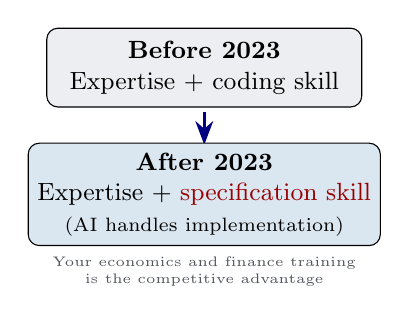
\begin{tikzpicture}[scale=0.7, every node/.style={font=\small}]
    \node[draw, rounded corners, fill=uzhgreylight, minimum width=4cm,
          minimum height=1cm, align=center] (old) at (0,3.8)
          {\textbf{Before 2023}\\Expertise + coding skill};
    \draw[-{Stealth[length=3mm]}, very thick, uzhblue] (0,3.0) -- (0,2.4);
    \node[draw, rounded corners, fill=softblue!20, minimum width=4cm,
          minimum height=1.3cm, align=center] (new) at (0,1.5)
          {\textbf{After 2023}\\Expertise + \emphc{specification skill}\\{\scriptsize (AI handles implementation)}};
    \node[font=\tiny, text=uzhgreydark, align=center] at (0,0.1)
          {Your economics and finance training\\is the competitive advantage};
\end{tikzpicture}
\end{center}

\vspace{0.3em}
\begin{block}{\small Key Insight}
\scriptsize
All AI coding tools use the same underlying models. The difference is \emphc{scaffolding}---how much environment access the agent has---not raw intelligence.
\end{block}
\end{columns}
\end{frame}

% --- AI Landscape ---
\begin{frame}{The AI Landscape: Three Major Players}
\scriptsize
\textbf{\textcolor{darkred}{Snapshot as of early 2026 \(\bullet\) semi-subjective \(\bullet\) re-check before re-using.}}\\
Frontier models, pricing, and rankings change on a monthly cadence. Treat this
slide as a working opinion, not a benchmark.

\vspace{0.2em}
\begin{columns}[T]
\column{0.32\textwidth}
\textbf{ChatGPT} \hfill \emph{OpenAI}
\begin{itemize}\itemsep0pt
  \item Strong math \& analytical reasoning
  \item Broadest ecosystem (voice, GPTs, Codex)
  \item Default general-purpose assistant
\end{itemize}

\column{0.32\textwidth}
\textbf{Claude} \hfill \emph{Anthropic}
\begin{itemize}\itemsep0pt
  \item Excellent writing, editing, close reading
  \item Very strong coding and project work
  \item Mature terminal agent via \texttt{claude code}
\end{itemize}

\column{0.32\textwidth}
\textbf{Gemini} \hfill \emph{Google}
\begin{itemize}\itemsep0pt
  \item Strong on long files and multimodal input
  \item Tight Google ecosystem integration
  \item Good if you live in Docs/Drive/Gmail
\end{itemize}
\end{columns}

\vspace{0.3em}
\begin{center}
\renewcommand{\arraystretch}{1.0}
\begin{tabular}{l c c c}
\toprule
\textbf{Task} & \textbf{ChatGPT / Codex} & \textbf{Claude} & \textbf{Gemini} \\
\midrule
Math \& analytical reasoning & \textcolor{darkgreen}{\checkmark\checkmark} & \textcolor{softorange}{\checkmark\checkmark} & \checkmark \\
Writing \& editing & \checkmark & \textcolor{softorange}{\checkmark\checkmark} & \checkmark \\
Coding \& repo-level work & \checkmark & \textcolor{softorange}{\checkmark\checkmark} & \checkmark \\
Long files / large context & \checkmark & \textcolor{softorange}{\checkmark\checkmark} & \textcolor{softblue}{\checkmark\checkmark} \\
Google ecosystem tasks & --- & --- & \textcolor{softblue}{\checkmark\checkmark} \\
\bottomrule
\end{tabular}
\end{center}

\vspace{0.2em}
\emphc{Why Claude Code for this course:}
all three vendors ship comparable browser chatbots; the distinctive piece is the
terminal agent. Anthropic's \texttt{claude code} is the most mature in early
2026. Most concepts (skills, subagents, hooks, MCP) transfer to OpenAI Codex
CLI, Gemini CLI, Cursor agent mode, or Aider with minor syntax changes; pick
the leaderboard \emph{(SWE-Bench Verified, Aider polyglot, WebDev Arena)}
benchmark you trust and re-check quarterly.

\vspace{0.2em}
{\tiny \emph{Other notable players we are not covering:}
xAI Grok, Meta Llama, Mistral, DeepSeek, Qwen --- strong on specific axes
(open weights, on-device, Chinese-language) but less mature for
research-grade terminal agents at the time of writing.}
\end{frame}

% --- Chatbox vs Agentic ---
\begin{frame}{Chatbox vs.\ Agentic: A Useful Analogy}
\scriptsize
\begin{alertblock}{Paul Goldsmith-Pinkham (2026)}
\itshape
``Web-based AI is like exchanging emails with a smart person.
Claude Code is like having them sit next to you, coding while you talk.''
\end{alertblock}

\vspace{0.2em}
\begin{columns}[T]
\column{0.32\textwidth}
\textbf{Think} \hfill \emph{browser chat}
\begin{itemize}\itemsep0pt
  \item Ideation, explanations, feedback
  \item Task mostly in your head
  \item Usually copy--paste
\end{itemize}

\column{0.32\textwidth}
\textbf{Work With Files} \hfill \emph{desktop app}
\begin{itemize}\itemsep0pt
  \item Drop in PDFs, screenshots, spreadsheets
  \item Read \& draft around single files
  \item Still outside your project tree
\end{itemize}

\column{0.32\textwidth}
\textbf{Run Workflows} \hfill \emph{terminal agent}
\begin{itemize}\itemsep0pt
  \item Read, write, and execute code
  \item Best when reproducibility matters
  \item Treat it like a \emphc{fast junior RA}
\end{itemize}
\end{columns}

\vspace{0.4em}
\emphc{Today's goal:} get every one of you from browser-chatbot copy-paste to
a terminal agent working inside a real, version-controlled research project.
The next slide maps that progression onto five discrete levels.
\end{frame}

% --- Hierarchy ---
\begin{frame}{The Hierarchy of AI Coding Tools}
\scriptsize

\begin{center}
\renewcommand{\arraystretch}{1.1}
\begin{tabular}{c p{6.0cm} p{4.7cm}}
\toprule
\textbf{Level} & \textbf{Capability} & \textbf{Examples (early 2026)} \\
\midrule
\textbf{0--1} & Browser chatbot + copy-paste & ChatGPT, Claude.ai, Gemini \\
\textbf{2} & Inline IDE assistant & Copilot (autocomplete), Cursor (composer) \\
\rowcolor{softblue!10}
\textbf{3} & \textbf{Terminal agent / agent mode---full env.\ access} & \textbf{Claude Code}, Codex CLI, Cursor agent, Aider, Copilot agent \\
\rowcolor{softblue!10}
\textbf{4} & Level 3 + external tools via MCP & + Zotero, GitHub, HPC, Brave Search \\
\textbf{5} & Closed-loop autonomy with verifier (1--2 hrs) & \textbf{Ralph} loops, Cursor Background Agents \\
\bottomrule
\end{tabular}
\end{center}

\vspace{0.3em}
\begin{columns}[T]
\column{0.58\textwidth}
\textbf{What makes Level 3+ different from Level 0--2?}
\begin{itemize}\itemsep0pt
    \item Reads and writes files on your machine
    \item Executes code and sees the output
    \item Uses git: commit, branch, diff
    \item Installs packages, manages environments
    \item Iterates autonomously---fixes its own errors
\end{itemize}

\column{0.40\textwidth}
\begin{alertblock}{This Lecture}
\scriptsize
We get you to \textbf{Level 3--4}, with a taste of Level~5 (Ralph). The jump
from L2 to L3 is the largest productivity gain: L2 suggests edits, L3
\emphc{does the work}.
\end{alertblock}
\end{columns}
\end{frame}

% --- Context Window ---
\begin{frame}[fragile]{The Context Window --- The Most Important Mental Model}
\small
\begin{columns}[T]
\column{0.48\textwidth}
An LLM (large language model) has \emphc{no persistent memory}. Every message bundles the \textbf{entire conversation history}---your prompts, Claude's responses, every file read, every code output---into one large document sent to the model.

\vspace{0.3em}
This is the \emphc{context window}:

\vspace{0.2em}
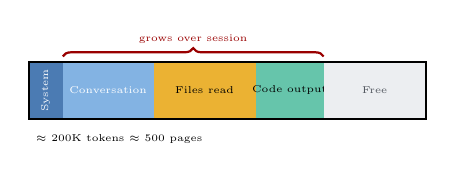
\begin{tikzpicture}[scale=0.72, transform shape]
    \def\barwidth{7}
    \def\barheight{1.0}
    \fill[level5!80] (0,0) rectangle (0.6,\barheight);
    \node[font=\tiny, text=white, rotate=90] at (0.3,0.5) {System};
    \fill[level3!80] (0.6,0) rectangle (2.2,\barheight);
    \node[font=\tiny, text=white] at (1.4,0.5) {Conversation};
    \fill[softorange!80] (2.2,0) rectangle (4.0,\barheight);
    \node[font=\tiny] at (3.1,0.5) {Files read};
    \fill[softgreen!60] (4.0,0) rectangle (5.2,\barheight);
    \node[font=\tiny] at (4.6,0.5) {Code output};
    \fill[uzhgreylight] (5.2,0) rectangle (\barwidth,\barheight);
    \node[font=\tiny, text=uzhgreydark] at (6.1,0.5) {Free};
    \draw[thick] (0,0) rectangle (\barwidth,\barheight);
    \node[font=\tiny, anchor=west] at (0,-0.35)
        {$\approx$ 200K tokens $\approx$ 500 pages};
    \draw[decorate, decoration={brace, amplitude=3pt}, thick, harvardcrimson]
        (0.6,\barheight+0.1) -- (5.2,\barheight+0.1)
        node[midway, above=3pt, font=\tiny, text=harvardcrimson] {grows over session};
\end{tikzpicture}

\vspace{0.3em}
\textbf{The performance curve:} Quality degrades as context fills. A session at turn~5 is sharper than the same session at turn~35.

\column{0.48\textwidth}
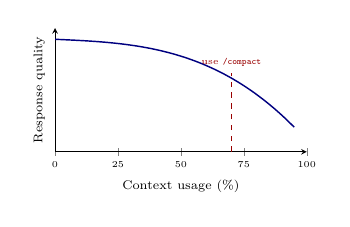
\begin{tikzpicture}[scale=0.65, transform shape]
\begin{axis}[
    width=6.5cm, height=4cm,
    xlabel={Context usage (\%)},
    ylabel={Response quality},
    xmin=0, xmax=100, ymin=0, ymax=1.1,
    xtick={0,25,50,75,100},
    ytick=\empty,
    axis lines=left,
    xlabel style={font=\scriptsize},
    ylabel style={font=\scriptsize},
    tick label style={font=\tiny},
    clip=false,
]
    \addplot[thick, uzhblue, smooth, domain=0:95]
        {1.0 - 0.1*(x/100) - 0.8*(x/100)^3};
    \draw[dashed, harvardcrimson, thick] (axis cs:70,0) -- (axis cs:70,0.7)
        node[above, font=\tiny, text=harvardcrimson] {use \texttt{/compact}};
\end{axis}
\end{tikzpicture}

\vspace{0.2em}
\textbf{Practical implications} (from Anthropic docs):
\begin{enumerate}\itemsep0pt
    \item[\scriptsize 1.] Break work into \emphc{focused sessions}
    \item[\scriptsize 2.] Write state to disk (\texttt{progress.md})
    \item[\scriptsize 3.] Use \texttt{/compact} before overflow
    \item[\scriptsize 4.] Fresh session (\texttt{/clear}) per sub-task
    \item[\scriptsize 5.] \emphc{Subagents} for research keep main context clean
\end{enumerate}

\vspace{0.1em}
{\tiny Boris Cherny: ``Context management is the single most critical resource.''}
\end{columns}
\end{frame}

% --- Task Taxonomy ---
\begin{frame}{Where AI Excels vs.\ Struggles}
\scriptsize
\begin{center}
\renewcommand{\arraystretch}{1.1}
\begin{tabular}{p{4.5cm} c p{4.5cm}}
\toprule
\textbf{Task Type} & \textbf{AI Quality} & \textbf{Notes} \\
\midrule
Data cleaning, reshaping & \textcolor{darkgreen}{\textbf{Excellent}} & Very fast ROI \\
Standard econometrics (OLS, GMM) & \textcolor{darkgreen}{\textbf{Excellent}} & Verify edge cases \\
Debugging cryptic errors & \textcolor{darkgreen}{\textbf{Excellent}} & Faster than Stack Overflow \\
Boilerplate (LaTeX, README) & \textcolor{darkgreen}{\textbf{Excellent}} & \\
Data analytics (SQL, dashboards) & \textcolor{darkgreen}{\textbf{Excellent}} & Use with CLI or MCP \\
\midrule
Novel theory derivation & \textcolor{darkred}{\textbf{Poor}} & Never trust without checking \\
Methods not in training data & \textcolor{softorange}{\textbf{Moderate}} & Degrades gracefully \\
Verification / self-checking & \textcolor{darkred}{\textbf{Poor}} & \emphc{Never skip human review} \\
Subtle identification issues & \textcolor{darkred}{\textbf{Poor}} & Economist must lead \\
\bottomrule
\end{tabular}
\end{center}

\vspace{0.2em}
\small
\begin{alertblock}{Key Insight (Bilionis replication experiment, 2026)}
\scriptsize
AI is a \emphc{very fast second-year PhD student}: excellent at known methods, mediocre at novel ones. Succeeded on in-distribution (SINDy), failed on out-of-distribution (unpublished BNN).
\end{alertblock}
\end{frame}

% --- The Master Workflow ---
\begin{frame}{The Master Workflow: Explore $\to$ Plan $\to$ Implement $\to$ Commit}

This four-phase workflow is the \emphc{single most important pattern} from the Anthropic docs and Boris Cherny's team. It applies to every non-trivial task.

\vspace{0.3em}
\begin{center}
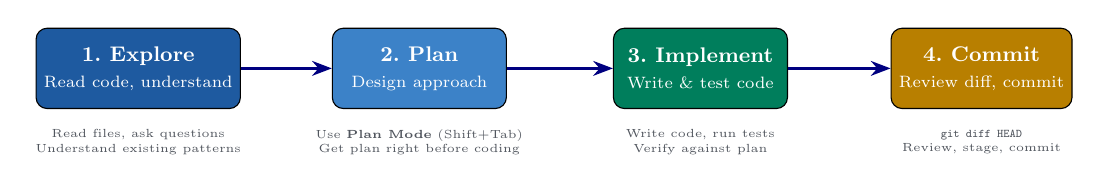
\begin{tikzpicture}[
    arr/.style={-{Stealth[length=2.5mm]}, very thick, uzhblue},
    scale=0.85, transform shape
]
    \node[cbox=level5] (explore) at (0,0) {\textbf{1.\ Explore}\\{\scriptsize Read code, understand}};
    \node[cbox=level4] (plan) at (4.2,0) {\textbf{2.\ Plan}\\{\scriptsize Design approach}};
    \node[cbox=softgreen!80!black] (impl) at (8.4,0) {\textbf{3.\ Implement}\\{\scriptsize Write \& test code}};
    \node[cbox=softorange!80!black] (commit) at (12.6,0) {\textbf{4.\ Commit}\\{\scriptsize Review diff, commit}};

    \draw[arr] (explore) -- (plan);
    \draw[arr] (plan) -- (impl);
    \draw[arr] (impl) -- (commit);

    \node[font=\tiny, text=uzhgreydark, align=center] at (0,-1.1)
        {Read files, ask questions\\Understand existing patterns};
    \node[font=\tiny, text=uzhgreydark, align=center] at (4.2,-1.1)
        {Use \textbf{Plan Mode} (Shift+Tab)\\Get plan right before coding};
    \node[font=\tiny, text=uzhgreydark, align=center] at (8.4,-1.1)
        {Write code, run tests\\Verify against plan};
    \node[font=\tiny, text=uzhgreydark, align=center] at (12.6,-1.1)
        {\texttt{git diff HEAD}\\Review, stage, commit};
\end{tikzpicture}
\end{center}

\vspace{0.3em}
\begin{columns}[T]
\column{0.48\textwidth}
\boristip{2} \textbf{Pour energy into the plan} so Claude can one-shot the implementation. If something goes sideways, switch \emph{back} to plan mode and re-plan instead of pushing through.

\column{0.48\textwidth}
\textbf{Skip planning only for:}
\begin{itemize}\itemsep0pt
    \item Single-line fixes (typos, obvious bugs)
    \item Adding a single function with clear requirements
    \item Tasks where you gave very specific instructions
\end{itemize}
\end{columns}
\end{frame}

% ============================================================================
% PART II: PRODUCTION ENVIRONMENT SETUP  (20 min)
% ============================================================================

\begin{frame}{}
\vfill
\begin{center}
{\Huge \textcolor{uzhblue}{\textbf{Part II}}}\\[12pt]
{\LARGE Production Environment Setup}\\[6pt]
{\small 20 minutes (includes Exercise 1)}
\end{center}
\vfill
\end{frame}

% --- Core Stack ---
\begin{frame}[fragile]{The Core Stack~\livedemo}
You need four things: a good terminal, Claude Code, version-control discipline, and Python.

\vspace{0.3em}
\begin{center}
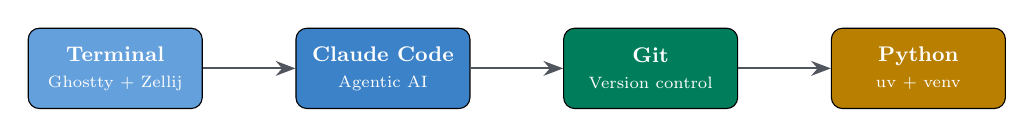
\begin{tikzpicture}[
    arr/.style={-{Stealth[length=2.5mm]}, thick, uzhgreydark},
    scale=0.85, transform shape
]
    \node[cbox=level3] (term) at (0,0) {\textbf{Terminal}\\{\scriptsize Ghostty + Zellij}};
    \node[cbox=level4] (claude) at (4,0) {\textbf{Claude Code}\\{\scriptsize Agentic AI}};
    \node[cbox=softgreen!80!black] (git) at (8,0) {\textbf{Git}\\{\scriptsize Version control}};
    \node[cbox=softorange!80!black] (python) at (12,0) {\textbf{Python}\\{\scriptsize uv + venv}};
    \draw[arr] (term) -- (claude);
    \draw[arr] (claude) -- (git);
    \draw[arr] (git) -- (python);
\end{tikzpicture}
\end{center}

\vspace{0.3em}
\begin{columns}[T]
\column{0.48\textwidth}
\begin{exampleblock}{Install (macOS / Linux)}
\begin{lstlisting}[style=bash, basicstyle=\scriptsize\ttfamily]
# Terminal (macOS: brew install ghostty)
# Claude Code
npm install -g @anthropic-ai/claude-code
# Python package manager
curl -LsSf https://astral.sh/uv/install.sh | sh
\end{lstlisting}
\end{exampleblock}

\column{0.48\textwidth}
\boristip{7} \textbf{Terminal setup tips:}
\begin{itemize}\itemsep0pt
    \item Use \texttt{/statusline} to show context usage and git branch
    \item Color-code terminal tabs by session purpose
    \item Voice dictation (fn$\times$2 on macOS)---you speak 3$\times$ faster than you type
    \item Use Zellij split panes: Claude $|$ Editor $|$ Output
\end{itemize}
\end{columns}
\end{frame}

% --- Self-study companion: Exercise 0 walk-through ---
\begin{frame}[fragile]{\selfstudy~~Exercise 0 ``Hello Claude'' --- What Success Looks Like}
\scriptsize
\textbf{Run before class} (or before reading further if self-study). Confirms install,
auth, and the basic ``read $\to$ write a file'' loop in one minute.

\vspace{0.3em}
\begin{columns}[T]
\column{0.48\textwidth}
\begin{exampleblock}{1. Verify the binary}
\begin{lstlisting}[style=bash, basicstyle=\tiny\ttfamily]
$ claude --version
1.x.y (Claude Code)
\end{lstlisting}
\end{exampleblock}

\begin{exampleblock}{2. Scratch folder + launch}
\begin{lstlisting}[style=bash, basicstyle=\tiny\ttfamily]
$ mkdir -p ~/research/hello-claude
$ cd ~/research/hello-claude
$ echo "Just testing." > notes.txt
$ claude
[Welcome to Claude Code]
\end{lstlisting}
\end{exampleblock}

\column{0.48\textwidth}
\begin{exampleblock}{3. Paste this prompt}
\begin{lstlisting}[style=prompt, basicstyle=\tiny\ttfamily]
> What files are in this directory?
  Then read notes.txt and rewrite
  it as a one-sentence haiku.
  Save to haiku.md.
\end{lstlisting}
\end{exampleblock}

\begin{exampleblock}{4. Expected response (paraphrased)}
\begin{lstlisting}[style=bash, basicstyle=\tiny\ttfamily]
I see notes.txt. Reading it...
"Just testing." -- writing haiku to haiku.md.
Done. Run `cat haiku.md` to see it.
\end{lstlisting}
\end{exampleblock}
\end{columns}

\vspace{0.2em}
\textbf{Troubleshooting:}
\textit{not found} $\Rightarrow$ \texttt{npm install -g @anthropic-ai/claude-code}; re-open terminal.~~
\textit{auth prompt} $\Rightarrow$ run \texttt{claude} again, browser opens for OAuth.
\end{frame}

% --- Claude Desktop modes ---
\begin{frame}{Claude Desktop: Chat, Cowork, Code}
\small
Before the terminal agent, know the three modes inside the \texttt{claude.ai}
desktop app. You will use all three during a typical research day.

\vspace{0.4em}
\begin{columns}[T]
\column{0.32\textwidth}
\begin{block}{\centering Chat}
\scriptsize
\begin{itemize}\itemsep1pt
  \item Standard conversational interface
  \item Brainstorm, summarize, explain
  \item Upload PDFs, images
  \item Same as \texttt{claude.ai} in the browser
\end{itemize}
\vspace{0.2em}
\emphc{Use for:} ideation before you touch any code.
\end{block}

\column{0.32\textwidth}
\begin{block}{\centering Cowork}
\scriptsize
\begin{itemize}\itemsep1pt
  \item ``Claude Code for non-developers''
  \item Agentic: \emph{executes} tasks, not just discusses them
  \item Organises files, analyzes spreadsheets, generates reports
  \item Can operate desktop apps on your behalf
\end{itemize}
\vspace{0.2em}
\emphc{Use for:} admin, light data work without a terminal.
\end{block}

\column{0.32\textwidth}
\begin{block}{\centering Code}
\scriptsize
\begin{itemize}\itemsep1pt
  \item The terminal agent (\texttt{claude code})
  \item Full file-system access
  \item Reads, writes, and runs code
  \item Most powerful mode for research projects
\end{itemize}
\vspace{0.2em}
\emphc{Use for:} everything reproducible.
\end{block}
\end{columns}

\vspace{0.4em}
\begin{alertblock}{Model selection (all three modes)}
\scriptsize
Switch between \textbf{Opus} (smartest, higher token cost) and \textbf{Sonnet}
(fast, cheaper, excellent for most tasks) with \texttt{/model} mid-session.
Use \textbf{Haiku} for cheap verifier subagents. Same models across Chat,
Cowork, and Code.
\end{alertblock}
\end{frame}

% --- Claude Code Setup ---
\begin{frame}[fragile]{Claude Code: First Launch \& Key Commands}
\begin{columns}[T]
\column{0.48\textwidth}
\begin{lstlisting}[style=bash, basicstyle=\scriptsize\ttfamily]
# Launch in your project
cd ~/research/my-project
claude

# Bootstrap project memory
/init

# Check your setup
/model
/cost
\end{lstlisting}

\vspace{0.3em}
\textbf{Subscription tiers} (2026):

\scriptsize
\renewcommand{\arraystretch}{1.05}
\begin{tabular}{lrl}
\toprule
\textbf{Tier} & \textbf{Price} & \textbf{Use case} \\
\midrule
Pro & \$20/mo & Getting started \\
Max 5x & \$100/mo & Daily research \\
Max 20x & \$200/mo & Multi-session, autonomous \\
Team & \$30/seat & Lab / co-author group \\
Enterprise & custom & SSO, ZDR, audit logs \\
API & \$15--75/MTok & Pay-per-use \\
\bottomrule
\end{tabular}

\column{0.48\textwidth}
\textbf{Essential commands:}

\vspace{0.2em}
\scriptsize
\renewcommand{\arraystretch}{1.15}
\begin{tabular}{ll}
\toprule
\textbf{Command} & \textbf{Purpose} \\
\midrule
\texttt{/help} & List all commands \\
\texttt{/model} & Switch model mid-session \\
\texttt{/cost} & Token spend so far \\
\texttt{/compact} & Compress conversation \\
\texttt{/clear} & Fresh context \\
\texttt{/init} & Bootstrap CLAUDE.md \\
\texttt{/agents} & Manage subagents \\
\texttt{/permissions} & Tool-allow rules \\
\texttt{Ctrl+C} & Interrupt execution \\
\texttt{ESC} & Cancel / undo turn \\
\texttt{ESC}$\times$2 & Rewind to checkpoint \\
\texttt{Shift+Tab} & Toggle Plan Mode \\
\bottomrule
\end{tabular}

\normalsize
\vspace{0.3em}
\begin{alertblock}{Privacy}
\scriptsize
Files stay local, but anything Claude \emphc{reads} enters the API context. Protect sensitive files with a \texttt{CLAUDE.md} rule (``never read \texttt{data/raw/}'') plus a \texttt{PreToolUse} hook (Part~VI) that hard-blocks the path.
\end{alertblock}
\end{columns}
\end{frame}

% --- Git Discipline ---
\begin{frame}[fragile]{Git: Your Safety Net}
AI-generated changes that are not version-controlled \emphc{cannot be rolled back}. Git is non-negotiable.

\vspace{0.3em}
\begin{columns}[T]
\column{0.48\textwidth}
\begin{lstlisting}[style=bash, basicstyle=\scriptsize\ttfamily]
# Create a research project
mkdir ~/research/my-paper
cd ~/research/my-paper
git init && git branch -M main

# Protect sensitive paths via CLAUDE.md
# (and a PreToolUse hook -- see Part VI)
cat > CLAUDE.md << 'EOF'
## Read-only paths
- data/raw/      # raw sensitive data
- .env           # API keys
- credentials/
EOF

# Create structure + first commit
mkdir -p {data/{raw,processed},
          code,figures,paper,notes}
git add . && git commit -m "initial"
\end{lstlisting}

\column{0.48\textwidth}
\textbf{The Git discipline cycle:}

\begin{center}
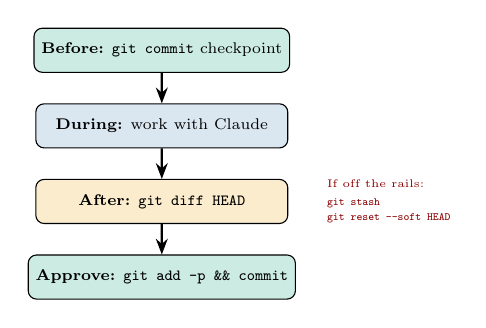
\begin{tikzpicture}[
    arr/.style={-{Stealth[length=2mm]}, thick},
    scale=0.8, transform shape
]
    \node[phase=softgreen!20] (pre) at (0,3.6)
        {\textbf{Before:} \texttt{git commit} checkpoint};
    \node[phase=softblue!20] (work) at (0,2.4)
        {\textbf{During:} work with Claude};
    \node[phase=softorange!20] (review) at (0,1.2)
        {\textbf{After:} \texttt{git diff HEAD}};
    \node[phase=softgreen!20] (commit) at (0,0)
        {\textbf{Approve:} \texttt{git add -p \&\& commit}};
    \draw[arr] (pre) -- (work);
    \draw[arr] (work) -- (review);
    \draw[arr] (review) -- (commit);
    \node[font=\tiny, text=darkred, align=left, anchor=west] at (2.5,1.2)
        {If off the rails:\\[2pt]\texttt{git stash}\\[1pt]\texttt{git reset --soft HEAD}};
\end{tikzpicture}
\end{center}

\vspace{0.2em}
{\scriptsize Before every session: commit. After every session: review the diff. Takes 30 seconds; makes everything recoverable.}
\end{columns}
\end{frame}

% --- MCP ---
\begin{frame}[fragile]{MCP: Connecting Claude to External Tools}
\small
\textbf{Model Context Protocol} (MCP) connects Claude to external services, turning it from Level~3 to Level~4.

\vspace{0.3em}
\begin{columns}[T]
\column{0.48\textwidth}
\begin{lstlisting}[style=bash, basicstyle=\scriptsize\ttfamily]
# Install MCP servers
claude mcp add zotero       # references
claude mcp add github       # PRs, issues
claude mcp add brave-search # web search
claude mcp add filesystem   # extended I/O
\end{lstlisting}

\vspace{0.2em}
\textbf{Usage in a session:}
\begin{lstlisting}[style=prompt, basicstyle=\scriptsize\ttfamily]
> Search Zotero for papers on
  carbon taxation in OLG models
> Create a GitHub branch called
  feature/robustness-checks
\end{lstlisting}

\vspace{0.2em}
\boristip{9} Use Claude with the \texttt{bq} CLI (or any database CLI/MCP) to pull and analyze metrics. Boris says he hasn't written SQL in 6+ months.

\column{0.48\textwidth}
\begin{center}
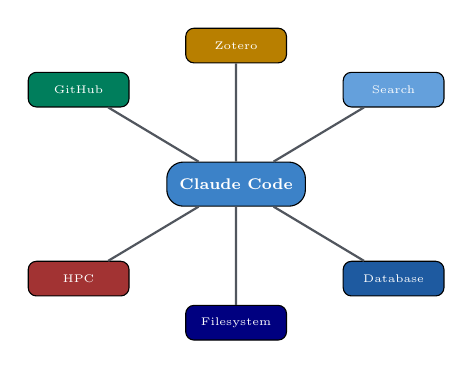
\begin{tikzpicture}[
    conn/.style={thick, uzhgreydark},
    scale=0.8, transform shape
]
    \node[draw, rounded corners=6pt, fill=level4,
          minimum width=2.2cm, minimum height=0.7cm,
          font=\scriptsize\bfseries, text=white] (cc) at (0,0) {Claude Code};

    \node[spoke=softgreen!80!black] (git) at (-2.5,1.5) {GitHub};
    \node[spoke=softorange!80!black] (zot) at (0,2.2) {Zotero};
    \node[spoke=level3] (search) at (2.5,1.5) {Search};
    \node[spoke=darkred!80] (hpc) at (-2.5,-1.5) {HPC};
    \node[spoke=uzhblue] (fs) at (0,-2.2) {Filesystem};
    \node[spoke=level5] (db) at (2.5,-1.5) {Database};

    \draw[conn] (cc) -- (git);
    \draw[conn] (cc) -- (zot);
    \draw[conn] (cc) -- (search);
    \draw[conn] (cc) -- (hpc);
    \draw[conn] (cc) -- (fs);
    \draw[conn] (cc) -- (db);
\end{tikzpicture}
\end{center}

\vspace{0.2em}
{\scriptsize Each MCP server runs locally and communicates via JSON-RPC. Claude calls tools through the server; your data never leaves your machine except through the API call itself.}
\end{columns}
\end{frame}

% --- Exercise 1 ---
\begin{frame}[fragile]{Exercise 1: Environment Bootstrap {\small(15 min)}}
\small
\begin{exampleblock}{Goal}
Get a working Claude Code session in a version-controlled project.
\end{exampleblock}

\begin{columns}[T]
\column{0.55\textwidth}
\begin{enumerate}\itemsep1pt
    \item Create directory: \texttt{mkdir \~{}/research/lecture-demo}
    \item Copy \texttt{lectures/lecture\_06\_B17\_agentic\_programming/code/generate\_synthetic\_data.py} and run it once
    \item Initialize git: \texttt{git init \&\& git branch -M main}
    \item Launch Claude: \texttt{claude}
    \item Run \texttt{/init} to bootstrap CLAUDE.md
    \item Type: \texttt{> What files are in this directory?}
    \item Type: \texttt{> Create explore\_data.py for data/synthetic\_panel.csv. Use pathlib.}
    \item Inspect the file. Run it on \texttt{data/synthetic\_panel.csv}.
    \item \texttt{git add . \&\& git commit -m "exercise 1"}
\end{enumerate}

\column{0.42\textwidth}
\textbf{Success criteria:}
\begin{itemize}\itemsep1pt
    \item[\textcolor{darkgreen}{\checkmark}] Claude Code running
    \item[\textcolor{darkgreen}{\checkmark}] Git repo with $\geq 1$ commit
    \item[\textcolor{darkgreen}{\checkmark}] CLAUDE.md exists
    \item[\textcolor{darkgreen}{\checkmark}] Python file runs
\end{itemize}

\vspace{0.3em}
\textbf{Troubleshooting:}
\begin{itemize}\itemsep0pt
    \item \texttt{claude: not found} $\to$ reinstall
    \item Auth error $\to$ \texttt{claude auth}
\end{itemize}

\vspace{0.3em}
{\scriptsize See \texttt{lectures/lecture\_06\_B17\_agentic\_programming/code/exercise\_prompts.md} for copy-pasteable prompts.}
\end{columns}
\end{frame}

% --- Self-study companion: full Ex 1 transcript ---
\begin{frame}[fragile]{\selfstudy~~Exercise 1: A Full Worked Session}
\scriptsize
What a healthy first run looks like, end to end. Blue = you; green = Claude.

\vspace{0.2em}
\begin{columns}[T]
\column{0.49\textwidth}
\begin{block}{\color{white}\bfseries Turn 1 -- you}
\begin{lstlisting}[style=prompt, basicstyle=\tiny\ttfamily]
> What files are in this directory?
  Summarize the structure.
\end{lstlisting}
\end{block}

\begin{exampleblock}{\color{white}\bfseries Turn 2 -- Claude}
\begin{lstlisting}[style=bash, basicstyle=\tiny\ttfamily]
[Listed: data/synthetic_panel.csv
 (5000 x 6: firm_id, year, revenue,
  employees, treated, post)]
One CSV: balanced panel of 500
firms x 10 years; 2015 treatment.
No code yet.
\end{lstlisting}
\end{exampleblock}

\column{0.49\textwidth}
\begin{block}{\color{white}\bfseries Turn 3 -- you}
\begin{lstlisting}[style=prompt, basicstyle=\tiny\ttfamily]
> Create explore_data.py: takes a
  CSV path on the CLI; prints shape,
  dtypes, first 5 rows, summary
  stats, % missing. Use pathlib.
  Add __main__ guard.
\end{lstlisting}
\end{block}

\begin{exampleblock}{\color{white}\bfseries Turn 4 -- Claude}
\begin{lstlisting}[style=bash, basicstyle=\tiny\ttfamily]
[Wrote explore_data.py]
[Ran python3 explore_data.py
        data/synthetic_panel.csv]
shape (5000, 6)  missing 0/6
revenue mean=10.32  sd=0.45
First 5 rows: [...]
\end{lstlisting}
\end{exampleblock}
\end{columns}

\vspace{0.3em}
{\tiny \textbf{What you should observe.} Claude (a) inspected before writing,
(b) satisfied every spec item in one pass, (c) ran the script itself.
\emph{If your session looks like this, your environment is healthy --- ready for Ex~2.}}
\end{frame}

% ============================================================================
% PART III: THE CORE INTERACTION LOOP  (20 min)
% ============================================================================

\begin{frame}{}
\vfill
\begin{center}
{\Huge \textcolor{uzhblue}{\textbf{Part III}}}\\[12pt]
{\LARGE The Core Interaction Loop}\\[6pt]
{\small 20 minutes (includes Exercise 2)}
\end{center}
\vfill
\end{frame}

% --- Feedback Loop ---
\begin{frame}{The Core Feedback Loop~\livedemo}
\begin{columns}[T]
\column{0.50\textwidth}
\begin{center}
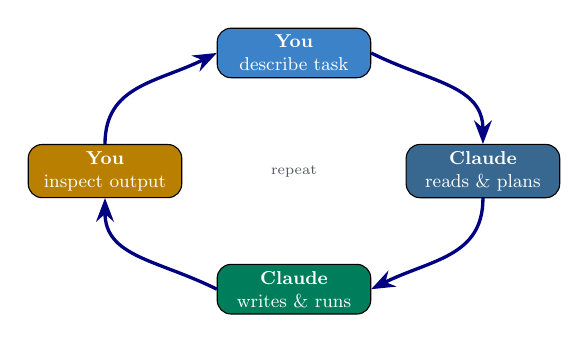
\begin{tikzpicture}[
    arr/.style={-{Stealth[length=3mm]}, very thick, uzhblue},
    scale=0.75, transform shape
]
    \node[fblock=level4] (you) at (0,2.5) {\textbf{You}\\describe task};
    \node[fblock=softblue!80!black] (read) at (3.2,0.5) {\textbf{Claude}\\reads \& plans};
    \node[fblock=softgreen!80!black] (write) at (0,-1.5) {\textbf{Claude}\\writes \& runs};
    \node[fblock=softorange!80!black] (inspect) at (-3.2,0.5) {\textbf{You}\\inspect output};

    \draw[arr] (you.east) .. controls +(1,-0.5) and +(0,1) .. (read.north);
    \draw[arr] (read.south) .. controls +(0,-1) and +(1,0.5) .. (write.east);
    \draw[arr] (write.west) .. controls +(-1,0.5) and +(0,-1) .. (inspect.south);
    \draw[arr] (inspect.north) .. controls +(0,1) and +(-1,-0.5) .. (you.west);

    \node[font=\scriptsize, text=uzhgreydark] at (0,0.5) {repeat};
\end{tikzpicture}
\end{center}

\column{0.47\textwidth}
\textbf{The most important skill: \emphc{how to interrupt.}}

\vspace{0.3em}
\renewcommand{\arraystretch}{1.2}
\begin{tabular}{ll}
\texttt{Ctrl+C} & Stop execution \\
\texttt{ESC} $\times 1$ & Cancel current message \\
\texttt{ESC} $\times 2$ & Rewind to checkpoint \\
\texttt{/rewind} & Go back N turns \\
\end{tabular}

\vspace{0.5em}
Do \emphc{not} let Claude finish a bad path and then course-correct. Interrupt early. After two failed corrections, \texttt{/clear} and write a better prompt from scratch.

\vspace{0.3em}
\boristip{5} \textbf{Claude fixes most bugs by itself.} Paste a Slack bug thread and say ``fix.'' Or say ``Go fix the failing CI tests.'' Don't micromanage \emph{how}.
\end{columns}
\end{frame}

% --- Self-study companion: feedback loop transcript ---
\begin{frame}[fragile]{\selfstudy~~The Feedback Loop in Action}
\scriptsize
One iteration condensed. Blue = you; green = Claude; orange = you steering.

\vspace{0.3em}
\begin{block}{\color{white}\bfseries 1. You describe the task}
\begin{lstlisting}[style=prompt, basicstyle=\tiny\ttfamily]
> data/synthetic_panel.csv has firm-year revenue.
  Print the sample mean per year. Use pandas. No plot yet.
\end{lstlisting}
\end{block}

\begin{exampleblock}{\color{white}\bfseries 2. Claude reads, writes, runs}
\begin{lstlisting}[style=bash, basicstyle=\tiny\ttfamily]
[Reads synthetic_panel.csv -- 5000x6]  [Writes scripts/year_means.py]
[Runs python3 scripts/year_means.py]
2010  9.95  2012 10.18  2014 10.31  2016 10.45  2018 10.55
2011 10.02  2013 10.25  2015 10.38  2017 10.50  2019 10.62
\end{lstlisting}
\end{exampleblock}

\begin{alertblock}{\color{white}\bfseries 3. You inspect, catch a bug, steer}
\begin{lstlisting}[style=prompt, basicstyle=\tiny\ttfamily]
> The 2015 jump looks suspicious -- is revenue already in logs?
  Print the column dtype and first 3 rows before the means.
\end{lstlisting}
\end{alertblock}

\vspace{0.1em}
{\tiny \textbf{Lesson:} steer between turns, not after a long bad path. Had turn~3 been ``great, now make a 4-panel figure,'' the bug from turn~2 would have silently propagated.}
\end{frame}

% --- Prompt Quality ---
\begin{frame}[fragile]{Prompt Quality Spectrum}
\small

Every research prompt exists on a spectrum from vague to precise. \emphc{Level 3 is always the goal.}

\vspace{0.3em}
\small
\renewcommand{\arraystretch}{1.3}
\begin{tabular}{c p{3cm} p{7.5cm}}
\toprule
\textbf{Level} & \textbf{Type} & \textbf{Example} \\
\midrule
\textcolor{darkred}{\textbf{0}} & Vague & \texttt{> Analyze this data} \\
\textbf{1} & Specific & \texttt{> Load gdp.csv. Compute YoY growth rates.} \\
\textbf{2} & + Context & \texttt{> Column `gdp\_real' is in 2015 USD billions, quarterly.} \\
\rowcolor{softgreen!10}
\textcolor{darkgreen}{\textbf{3}} & \textbf{+ Constraints + Output + Verify} & \texttt{> Use .iloc not .ix. Write to processed/. Output: Markdown table. Flag outliers $>$10\%. Assert N $>$ 1000.} \\
\bottomrule
\end{tabular}

\vspace{0.3em}
\begin{columns}[T]
\column{0.48\textwidth}
\textbf{What makes Level 3 different:}
\begin{itemize}\itemsep0pt
    \item Exact file paths and column names
    \item Formula or method specified explicitly
    \item Negative constraints (what NOT to do)
    \item Output format defined
    \item Verification step included
\end{itemize}

\column{0.48\textwidth}
\boristip{6} \textbf{Challenge Claude:}
\begin{itemize}\itemsep0pt
    \item ``Grill me on these changes and don't make a PR until I pass your test.''
    \item ``Knowing everything you know now, scrap this and implement the elegant solution.''
    \item Specificity is not nagging---it is the entire skill.
\end{itemize}
\end{columns}
\end{frame}

% --- Level 3 Example ---
\begin{frame}[fragile]{A Level 3 Prompt in Detail~\livedemo}
\begin{lstlisting}[style=prompt, basicstyle=\scriptsize\ttfamily]
> Load data/gdp_quarterly.csv.
  - Column 'gdp_real': real GDP in 2015 USD billions, quarterly.
  - Compute year-over-year growth: g_t = (gdp_t / gdp_{t-4}) - 1
  - Print a summary table with: mean, sd, p5, p95, N
  - Flag quarters where |g_t| > 0.1 as outliers, print a list
  - Write the cleaned series to data/processed/gdp_growth.csv
  - Do NOT use pandas deprecated methods -- use .iloc, not .ix
  Expected output format: Markdown table printed to stdout.
\end{lstlisting}

\vspace{0.3em}
\begin{columns}[T]
\column{0.48\textwidth}
\textbf{Checklist---what makes this Level 3:}
\begin{itemize}\itemsep1pt
    \item[\checkmark] Exact file path \& column name
    \item[\checkmark] Formula specified ($g_t$)
    \item[\checkmark] Output statistics listed
    \item[\checkmark] Outlier threshold given
    \item[\checkmark] Output path specified
    \item[\checkmark] Negative constraint (no deprecated API)
    \item[\checkmark] Expected output format
\end{itemize}

\column{0.48\textwidth}
\textbf{Common research task patterns:}
\begin{itemize}\itemsep2pt
    \item[\textbf{A}] ``Explain what this code does''
    \item[\textbf{B}] ``Write code matching existing style''
    \item[\textbf{C}] ``Debug this error''
    \item[\textbf{D}] ``Refactor for reproducibility''
    \item[\textbf{E}] ``Generate a LaTeX table''
\end{itemize}

\vspace{0.3em}
{\small See exercise handout for full templates of each pattern.}
\end{columns}
\end{frame}

% --- Self-study companion: what Claude returns to the Level 3 prompt ---
\begin{frame}[fragile]{\selfstudy~~Claude's Response to the Level-3 Prompt}
\scriptsize
After ${\sim}40$ seconds Claude reads the file, writes the script, runs it,
prints the summary, and persists the cleaned series.

\vspace{0.2em}
\begin{columns}[T]
\column{0.50\textwidth}
\begin{exampleblock}{Terminal output (abridged)}
\begin{lstlisting}[style=bash, basicstyle=\tiny\ttfamily]
[Read gdp_quarterly.csv -- 320 rows]
[Wrote scripts/gdp_growth.py]
[Ran python3 scripts/gdp_growth.py]

stat   mean    sd     p5     p95   N
value  0.0205  0.018 -0.008  0.049 316

Outliers (|g_t| > 0.10):
  2008Q4: -0.121
  2020Q2: -0.219
  2020Q3:  0.156

[Wrote processed/gdp_growth.csv]
\end{lstlisting}
\end{exampleblock}

\column{0.48\textwidth}
\textbf{End to end, in one pass:}
\begin{enumerate}\itemsep0pt
    \item Read the raw CSV; inspected schema.
    \item Wrote \texttt{scripts/gdp\_growth.py}.
    \item Ran it; saw the table.
    \item Persisted the cleaned series.
    \item Surfaced three outliers at your threshold.
\end{enumerate}

\vspace{0.2em}
\begin{block}{Why this is Level 3}
\tiny
No re-prompt for the table, no re-prompt for the file write, no re-prompt for
outliers. Each was \emph{specified up-front}; Claude satisfied all six
checklist items in one pass.
\end{block}
\end{columns}
\end{frame}

% --- Parallel Sessions ---
\begin{frame}[fragile]{Parallel Sessions \& Worktrees}
\boristip{1} \textbf{Do more in parallel.} This is the single biggest productivity unlock from the Claude Code team.

\vspace{0.3em}
\begin{columns}[T]
\column{0.48\textwidth}
Spin up 3--5 git \emphc{worktrees}, each running its own Claude session:

\begin{lstlisting}[style=bash, basicstyle=\scriptsize\ttfamily]
# Create worktrees
git worktree add ../proj-a -b data-clean
git worktree add ../proj-b -b estimation
git worktree add ../proj-c -b lit-review

# Launch Claude in each
cd ../proj-a && claude  # Terminal 1
cd ../proj-b && claude  # Terminal 2
cd ../proj-c && claude  # Terminal 3
\end{lstlisting}

\vspace{0.2em}
{\scriptsize Worktrees share repo state (unlike clones), reducing merge conflicts. Each session works on non-overlapping files.}

\column{0.48\textwidth}
\begin{center}
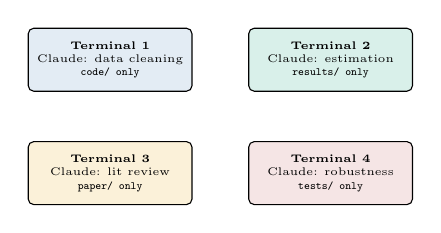
\begin{tikzpicture}[scale=0.8, transform shape]
    \node[tpane=softblue!15] (t1) at (0,0)
        {\textbf{Terminal 1}\\Claude: data cleaning\\{\ttfamily code/ only}};
    \node[tpane=softgreen!15] (t2) at (3.5,0)
        {\textbf{Terminal 2}\\Claude: estimation\\{\ttfamily results/ only}};
    \node[tpane=softorange!15] (t3) at (0,-1.8)
        {\textbf{Terminal 3}\\Claude: lit review\\{\ttfamily paper/ only}};
    \node[tpane=harvardcrimson!10] (t4) at (3.5,-1.8)
        {\textbf{Terminal 4}\\Claude: robustness\\{\ttfamily tests/ only}};
\end{tikzpicture}
\end{center}

\vspace{0.2em}
\textbf{Key:} Set scope explicitly in each session:
\begin{lstlisting}[style=prompt, basicstyle=\tiny\ttfamily]
> You are only allowed to modify
  files in the code/ directory.
\end{lstlisting}

\vspace{0.2em}
{\tiny\textcolor{darkred}{\textbf{Cost warning:}} 3--5 sessions consume API
quota in parallel. On Pro (\$20/mo) you will hit limits within minutes; Max
or API pay-as-you-go is the realistic tier here.}
\end{columns}
\end{frame}

% --- Context Management ---
\begin{frame}[fragile]{Context Management in Practice}
\begin{columns}[T]
\column{0.48\textwidth}
\textbf{The progress file pattern:}\\
{\small For any session $> 10$ turns.}

\begin{lstlisting}[style=prompt, basicstyle=\scriptsize\ttfamily]
> Write notes/session_state.md:
  1. What we have done so far
  2. What is working
  3. What we need to do next
  4. Design decisions and why
\end{lstlisting}

Next session:
\begin{lstlisting}[style=prompt, basicstyle=\scriptsize\ttfamily]
> Read notes/session_state.md and
  continue from where we left off.
\end{lstlisting}

\vspace{0.3em}
\textbf{Session resume options:}
\begin{itemize}\itemsep0pt
    \item \texttt{claude --continue} --- resume last session
    \item \texttt{claude --resume} --- pick from recent sessions
    \item \texttt{/rename "estimation pipeline"} --- name sessions for easy recall
\end{itemize}

\column{0.48\textwidth}
\textbf{When to use which approach:}

\vspace{0.2em}
\scriptsize
\renewcommand{\arraystretch}{1.2}
\begin{tabular}{p{2cm} p{4cm}}
\toprule
\textbf{Situation} & \textbf{Action} \\
\midrule
$<5$ turns & Just work directly \\
5--15 turns & Write progress file at end \\
$>15$ turns & \texttt{/compact} + progress file \\
New sub-task & \texttt{/clear} or new session \\
Research task & Use \emphc{subagent} to keep main context clean \\
\bottomrule
\end{tabular}

\normalsize
\vspace{0.3em}
\begin{alertblock}{\small Anthropic's \#1 Failure Pattern}
\scriptsize
\textbf{Kitchen-sink sessions:} mixing unrelated tasks in one session. Each task adds context that degrades all other tasks. Use \texttt{/clear} between unrelated work.
\end{alertblock}
\end{columns}
\end{frame}

% --- Exercise 2 ---
\begin{frame}[fragile]{Exercise 2: First Real Task {\small(15 min)}}
\begin{exampleblock}{Goal}
Use a Level 3 prompt on real data and practice context management.
\end{exampleblock}

\begin{lstlisting}[style=prompt, basicstyle=\scriptsize\ttfamily]
> I have a dataset at data/synthetic_panel.csv.
  Without loading it yet, first tell me how to inspect it.
  Then:
  1. Load it and print diagnostics (columns, shape, date range, missing)
  2. Compute annual average revenue by treatment group
  3. Generate a 2x2 panel of plots (matplotlib,
     publication-ready, no gridlines, serif font, 6x5 inches)
  4. Save the figure to figures/panel_overview.pdf
  5. Write a 3-sentence description to notes/data_description.md
\end{lstlisting}

\vspace{0.2em}
{\small No CSV? First run \texttt{python generate\_synthetic\_data.py} in the project root.}

\vspace{0.2em}
\textbf{Reflection:} Where did Claude do well? Where did it need correction? At what point would you have interrupted? What constraint would have prevented any issues?
\end{frame}

% ============================================================================
% PART IV: PROMPT ENGINEERING FOR RESEARCH  (20 min)
% ============================================================================

\begin{frame}{}
\vfill
\begin{center}
{\Huge \textcolor{uzhblue}{\textbf{Part IV}}}\\[12pt]
{\LARGE Prompt Engineering for Research}\\[6pt]
{\small 20 minutes (includes Exercise 3)}
\end{center}
\vfill
\end{frame}

% --- Prompt Anatomy ---
\begin{frame}{Anatomy of a Research Prompt}
\small
Every good research prompt has up to \emphc{six components}. Not every prompt needs all six---but omitting any one produces a specific failure mode.

\vspace{0.3em}
\begin{center}
\small
\renewcommand{\arraystretch}{1.2}
\begin{tabular}{c p{2.5cm} p{5cm} p{3.5cm}}
\toprule
\textbf{\#} & \textbf{Component} & \textbf{What it does} & \textbf{Failure if missing} \\
\midrule
1 & \textbf{ROLE} & Who Claude is in this task & Generic, non-expert output \\
2 & \textbf{CONTEXT} & What it needs to know & Asks too many questions \\
3 & \textbf{TASK} & What you want done & Invents a different task \\
4 & \textbf{CONSTRAINTS} & Must / must not do & ``AI's code'' not ``my code'' \\
5 & \textbf{OUTPUT} & Deliverable format & Wrong format, extra junk \\
6 & \textbf{VERIFICATION} & How to check it worked & Plausible but wrong \\
\bottomrule
\end{tabular}
\end{center}

\vspace{0.3em}
\begin{block}{The Meta-Rule}
When something goes wrong, ask: ``Which of the 6 components did I omit?'' The answer is almost always the fix.
\end{block}
\end{frame}

% --- Constraints ---
\begin{frame}[fragile]{The Constraint Vocabulary}
Constraints are the difference between ``AI wrote the code'' and ``AI wrote \emphc{my} code.''

\vspace{0.3em}
\begin{columns}[T]
\column{0.32\textwidth}
\textbf{\textcolor{darkred}{Negative}} (what NOT to do):
\begin{lstlisting}[style=prompt, basicstyle=\tiny\ttfamily]
Do NOT use statsmodels
  -- use linearmodels.
Do NOT change existing
  function signatures.
Do NOT use deprecated
  pandas syntax.
Do NOT hardcode file
  paths.
\end{lstlisting}

\column{0.32\textwidth}
\textbf{\textcolor{darkgreen}{Positive}} (what to do):
\begin{lstlisting}[style=prompt, basicstyle=\tiny\ttfamily]
Always use type hints.
Follow AEA data policy:
  reproducible from one
  script.
Use exact notation from
  paper/main.tex.
Maintain backward
  compatibility with
  test suite.
\end{lstlisting}

\column{0.32\textwidth}
\textbf{\textcolor{uzhblue}{Scope}} (boundaries):
\begin{lstlisting}[style=prompt, basicstyle=\tiny\ttfamily]
Only modify files in
  the code/ directory.
Do not touch paper/
  or data/raw/.
Make the minimum change
  needed to fix the bug.
Do one thing at a time;
  stop and report before
  the next step.
\end{lstlisting}
\end{columns}

\vspace{0.3em}
\begin{alertblock}{The ``Think Before You Code'' Pattern}
\small
For complex tasks, \emphc{force a planning step}: ``BEFORE writing any code: (1) Describe your plan, (2) List every file you'll modify, (3) List risks. Do not proceed until I say `go ahead.'\,'' This single pattern prevents $\sim$80\% of ``Claude rewrote everything'' disasters.
\end{alertblock}
\end{frame}

% --- Research Templates ---
\begin{frame}[fragile]{Research Prompt Templates}
\small
\begin{columns}[T]
\column{0.48\textwidth}
\textbf{Template 1: Replication Check}
\begin{lstlisting}[style=prompt, basicstyle=\tiny\ttfamily]
> Read code/estimate.py and
  paper/main.tex Sec 3.2--3.4.
  Check: does the code match
  the model in the paper?
  Write a discrepancy report:
  (*@\checkmark@*) [item]: matches
  (*@$\times$@*) [item]: paper says X, code does Y
  ? [item]: unclear from paper
\end{lstlisting}

\vspace{0.2em}
\textbf{Template 2: Robustness Table}
\begin{lstlisting}[style=prompt, basicstyle=\tiny\ttfamily]
> Add 3 robustness checks to Table 2.
  Baseline: code/estimate_baseline.py
  Specs: (1) add year FE
         (2) drop leverage > 0.9
         (3) winsorize at 1%/99%
  For each: separate script, save to
    results/robustness_{name}.json
  Then generate a LaTeX table with
  all 4 specs side by side (booktabs).
\end{lstlisting}

\column{0.48\textwidth}
\textbf{Template 3: Autonomous Session}
\begin{lstlisting}[style=prompt, basicstyle=\tiny\ttfamily]
> I'm stepping away for 30 minutes.
  Task: implement the pipeline
  per plan.md.
  Rules while I am away:
  - Commit after each major step
  - If stuck after 3 attempts,
    write to notes/blocked.md
    and STOP
  - Do NOT modify data/raw/
  - Write progress every 10 steps
    to notes/progress.md
  When done: summary to
    notes/session_end.md.
\end{lstlisting}

\vspace{0.2em}
\textbf{Template 4: Literature Writing}
\begin{lstlisting}[style=prompt, basicstyle=\tiny\ttfamily]
> Do NOT invent any citations.
  Only cite papers already in
  paper/references.bib.
  If not in bib, write:
  [CITE: author, year -- verify]
\end{lstlisting}
\end{columns}
\end{frame}

% --- Failure Modes ---
\begin{frame}{Common Failure Modes and Fixes}
\scriptsize
\begin{center}
\renewcommand{\arraystretch}{1.1}
\begin{tabular}{p{3.5cm} p{3cm} p{5cm}}
\toprule
\textbf{Failure} & \textbf{Cause} & \textbf{Fix} \\
\midrule
Claude ``invents'' results & Vague output spec & Add explicit verification step \\
Code works but unreadable & No style constraint & Specify style in role prompt \\
Modifies wrong files & No scope constraint & Add explicit file scope \\
Long session degrades & Context overflow & \texttt{/compact}, break into sessions \\
Loops on same error & No retry limit & ``If 3 attempts fail, stop'' \\
Wrong statistical method & Insufficient domain & Role prompt + method name \\
Output $\neq$ paper & Disconnected context & Point Claude to paper section \\
Over-specified CLAUDE.md & Too-long instructions & Keep CLAUDE.md $<200$ lines \\
\bottomrule
\end{tabular}
\end{center}

\vspace{0.2em}
\begin{columns}[T]
\column{0.58\textwidth}
\textbf{Top 3 anti-patterns (Anthropic docs):}
\begin{enumerate}\itemsep0pt
    \item \textbf{Kitchen-sink sessions:} mixing unrelated tasks
    \item \textbf{Correcting repeatedly} instead of starting fresh
    \item \textbf{Trust-then-verify gap:} no tests or expected outputs
\end{enumerate}

\column{0.38\textwidth}
\begin{block}{Highest-leverage fix}
\tiny
\emphc{Give Claude a way to verify its own work.} Tests, expected outputs, or synthetic data with known answers prevent most failures.
\end{block}
\end{columns}
\end{frame}

% --- Exercise 3 ---
\begin{frame}[fragile]{Exercise 3: Prompt Refactor {\small(15 min)}}
\begin{exampleblock}{Goal}
Take a bad prompt and improve it using the 6-component framework.
\end{exampleblock}

\textbf{Starting prompt} (Level 0---everything is wrong):
\begin{lstlisting}[style=prompt, basicstyle=\normalsize\ttfamily]
> Analyze the data and run the regression and make a table.
\end{lstlisting}

\vspace{0.3em}
\textbf{Your task:}
\begin{enumerate}\itemsep2pt
    \item \textbf{Diagnose:} Which of the 6 components are missing? (Answer: all of them.)
    \item \textbf{Rewrite:} Create a Level 3 version for your own research context.
    \item \textbf{Peer review:} Share with a neighbor and critique each other's prompts.
    \item \textbf{Test:} Run both versions and compare output quality.
\end{enumerate}

\vspace{0.2em}
\textbf{Bonus:} Take a prompt you've used in the past that produced disappointing results. Apply the 6-component framework and rerun it.
\end{frame}

% ============================================================================
% PART V: PROJECT MEMORY & CLAUDE.md  (15 min)
% ============================================================================

\begin{frame}{}
\vfill
\begin{center}
{\Huge \textcolor{uzhblue}{\textbf{Part V}}}\\[12pt]
{\LARGE Project Memory \& CLAUDE.md}\\[6pt]
{\small 15 minutes (includes Exercise 4)}
\end{center}
\vfill
\end{frame}

% --- CLAUDE.md ---
\begin{frame}{What is CLAUDE.md?}
\small
\texttt{CLAUDE.md} is read \emphc{automatically} at session start---your project's persistent memory for a capable but amnesiac research assistant.

\vspace{0.2em}
\begin{columns}[T]
\column{0.48\textwidth}
\textbf{Where:} \texttt{\~{}/.claude/CLAUDE.md} (user-global), \texttt{./CLAUDE.md} or \texttt{./.claude/CLAUDE.md} (project root), \texttt{subdir/CLAUDE.md} (path-scoped). All are loaded; nearest wins. Use \texttt{@path/to/file.md} to import shared rules across projects.

\vspace{0.2em}
\textbf{Highest-value sections:}
\begin{enumerate}\itemsep0pt
    \item Repository structure (read-only dirs)
    \item Coding standards
    \item Statistical conventions \& notation
    \item Current status (update each session)
    \item ``Do Not Touch'' list
\end{enumerate}

\column{0.48\textwidth}
\boristip{3} \textbf{Invest in your CLAUDE.md.} After every correction:

\vspace{0.1em}
\begin{center}
\fcolorbox{harvardcrimson}{red!5}{%
\parbox{5cm}{\centering\scriptsize\itshape
``Update CLAUDE.md so you don't\\make that mistake again.''}}
\end{center}

\vspace{0.1em}
{\scriptsize Claude is eerily good at writing rules for itself. Keep iterating until mistake rate drops.}

\vspace{0.2em}
\textbf{Best practices} (Reddit + Anthropic):
\begin{itemize}\itemsep0pt
    \item Keep root CLAUDE.md $<$200 lines
    \item Specific rules in subfolder files
    \item Use \texttt{.claude/rules/} for path-scoped rules
    \item Critical rules: use \emphc{hooks} (code enforcement)
\end{itemize}
\end{columns}
\end{frame}

% --- CLAUDE.md Template ---
\begin{frame}[fragile]{CLAUDE.md Template for Economics Research}
\begin{columns}[T]
\column{0.48\textwidth}
\begin{lstlisting}[style=bash, basicstyle=\tiny\ttfamily]
# CLAUDE.md -- [Paper Title]

## Project Overview
- **Topic:** [one sentence]
- **Stage:** draft / revision / final
- **Target journal:** [e.g., RES]

## Repository Structure
data/
  raw/        <- READ ONLY. Never modify.
  processed/  <- Your outputs go here
code/
  estimate.py <- Main estimation
  config.py   <- All parameters here
figures/      <- PDF format
paper/main.tex

## Coding Standards
- Python 3.11+; type hints on all sigs
- pathlib.Path for all file I/O
- Seeds: set in config.py, pass explicit
- PEP 8, max line length 88 (black)

## Statistical Conventions
- SEs: clustered at [firm] level
- FE: two-way (firm + year) baseline
\end{lstlisting}

\column{0.48\textwidth}
\begin{lstlisting}[style=bash, basicstyle=\tiny\ttfamily]
## Notation (matches paper/main.tex)
- i = firm, t = year
- Y_it = outcome variable
- D_it = treatment indicator
- beta = coefficient of interest

## What I Am Working On Now
[UPDATE THIS EVERY SESSION]
- Current task: ...
- Last completed: ...
- Next step: ...

## Do Not Touch
- data/raw/ -- needs confirmation
- Main estimation function signature
- Any file in paper/ without asking

## Known Pitfalls
- [AI mistakes to avoid -- add here]

## Decisions Made (and Why)
- Used OLS not IV because [reason]
\end{lstlisting}

\vspace{0.1em}
{\tiny Copy-pasteable version: \texttt{lectures/lecture\_06\_B17\_agentic\_programming/code/CLAUDE\_md\_template.md}}
\end{columns}
\end{frame}

% --- Three-Layer Architecture ---
\begin{frame}[fragile]{Three-Layer Architecture for AI-Assisted Projects}
\scriptsize
From the course's \texttt{utils-agentic-support} framework:

\vspace{0.3em}
\begin{center}
\small
\renewcommand{\arraystretch}{1.25}
\begin{tabular}{p{2.5cm} p{4cm} p{2.5cm} p{2.5cm}}
\toprule
\textbf{Layer} & \textbf{Purpose} & \textbf{Change Freq.} & \textbf{Who Edits} \\
\midrule
\textbf{Standards} & Human-readable guidelines (style, conventions, methodology) & Slow (quarterly) & Team review \\
\textbf{Runtime} & Machine-executable configs (CLAUDE.md, skills, subagents) & Fast (daily) & Individual \\
\textbf{Templates} & Project bootstrapping files & Moderate & Team \\
\bottomrule
\end{tabular}
\end{center}

\vspace{0.3em}
\begin{columns}[T]
\column{0.48\textwidth}
\textbf{Why this separation matters:}
\begin{itemize}\itemsep1pt
    \item Standards define \emph{how the team works}---style guides, coding conventions, research methodology
    \item Runtime files are what AI tools actually read and execute---they iterate quickly
    \item Templates bootstrap new projects with the right structure from day one
\end{itemize}

\column{0.48\textwidth}
\textbf{Distribution model:} Add as a git submodule:
\begin{lstlisting}[style=bash, basicstyle=\scriptsize\ttfamily]
git submodule add \
  https://github.com/your-org/
  agentic-support .agentic
\end{lstlisting}

\vspace{0.2em}
Projects reference shared standards but customize their own CLAUDE.md $\to$ organization-wide consistency + project-specific needs.
\end{columns}
\end{frame}

% --- Exercise 4 ---
\begin{frame}[fragile]{Exercise 4: Write Your Own CLAUDE.md {\small(10 min)}}
\begin{exampleblock}{Goal}
Create a CLAUDE.md for a real or hypothetical research project.
\end{exampleblock}

\begin{enumerate}\itemsep2pt
    \item Choose a project (your own, or the lecture demo)
    \item Copy the template from \texttt{lectures/lecture\_06\_B17\_agentic\_programming/code/CLAUDE\_md\_template.md}
    \item Fill in the \emphc{three highest-value sections}: Repository Structure, Coding Standards, Current Status
    \item Launch a fresh Claude session (\texttt{/clear})
    \item Type: \texttt{> Summarize this project and what I should work on next.}
    \item Observe how Claude uses the CLAUDE.md to orient itself
    \item Deliberately make Claude do something wrong, then tell it: ``Update CLAUDE.md so you don't make that mistake again.''
\end{enumerate}
\end{frame}

% ============================================================================
% PART VI: SKILLS, SUBAGENTS & HOOKS  (15 min)
% ============================================================================

\begin{frame}{}
\vfill
\begin{center}
{\Huge \textcolor{uzhblue}{\textbf{Part VI}}}\\[12pt]
{\LARGE Skills, Subagents \& Advanced Workflows}\\[6pt]
{\small 15 minutes (includes Exercise 5)}
\end{center}
\vfill
\end{frame}

% --- Skills vs Subagents vs MCP map ---
\begin{frame}[shrink=10]{Skills vs.\ Subagents vs.\ Hooks vs.\ MCP --- a Quick Map}
\scriptsize
Four extension mechanisms; each does one thing the others can't.

\vspace{0.3em}
\renewcommand{\arraystretch}{1.15}
\begin{tabular}{p{1.8cm} p{3.4cm} p{3.8cm} p{3.4cm}}
\toprule
\textbf{Mechanism} & \textbf{What it is} & \textbf{Lives at} & \textbf{Use when} \\
\midrule
\emphc{Skill} (Agent Skill, Oct 2025) &
  Multi-step \emph{workflow} as \texttt{SKILL.md}; invoked as a slash command. &
  \texttt{.claude/skills/<name>/SKILL.md} &
  Same prompt sequence $\geq$~daily. \\
\emphc{Subagent} &
  Specialized assistant (own model, tools, prompt); spawned via \texttt{Task}. &
  \texttt{.claude/agents/<name>.md} &
  Fresh context or different model for one sub-task. \\
\emphc{Hook} &
  Shell command fired around tool calls (\texttt{PreToolUse}, \texttt{Post\-ToolUse}, \texttt{Stop}, \dots). &
  \texttt{.claude/settings.json} &
  \emph{Deterministic} enforcement (block paths, lint, audit log). \\
\emphc{MCP server} &
  External service exposing tools (Zotero, GitHub, DBs) via MCP. &
  Out-of-process; \texttt{claude mcp add} &
  Data/actions outside the project tree. \\
\bottomrule
\end{tabular}

\vspace{0.3em}
\textbf{Rule of thumb.} Skills package prompts; subagents package specialists;
hooks enforce policy; MCP plugs in external worlds. \emphc{Ralph} (Part~VII)
wraps all four into a closed loop.

\vspace{0.1em}
{\tiny Refs: Schluntz \& Zhang (2024), ``Building Effective Agents''; Anthropic Agent Skills (Oct 2025); MCP \url{https://modelcontextprotocol.io}.}
\end{frame}

% --- Skills ---
\begin{frame}[fragile]{Custom Skills: Reusable Workflows as Slash Commands}
\scriptsize
\boristip{4} \textbf{If you do something more than once a day, turn it into a skill.}

\vspace{0.3em}
Skills are multi-step workflows saved as \texttt{SKILL.md} files in \texttt{.claude/skills/}. They can be invoked with a slash command.

\vspace{0.3em}
\begin{columns}[T]
\column{0.48\textwidth}
\textbf{Example: \texttt{/data-diagnostics}}

{\scriptsize File: \texttt{.claude/skills/data-diagnostics/}\\
\texttt{SKILL.md}}
\begin{lstlisting}[style=bash, basicstyle=\tiny\ttfamily]
---
name: data-diagnostics
description: Run quality checks on a CSV
---
# Data Diagnostics Skill

When invoked with a file path:
1. Load the file (do NOT modify it)
2. Print: shape, dtypes, date range
3. Print: % missing by column
4. Print: summary stats (mean, sd,
   p10, p25, p50, p75, p90)
5. Flag: duplicates, negatives where
   impossible, outliers > 5 SD
6. Save report to notes/data_report.md
\end{lstlisting}

\column{0.48\textwidth}
\textbf{Examples from production teams:}
\begin{itemize}\itemsep2pt
    \item \texttt{/commit} --- review changes, run pre-commit checks, stage, commit with conventional format, push, create PR
    \item \texttt{/simplify} --- post-implementation cleanup: reduce nesting, apply Pythonic patterns, remove dead code
    \item \texttt{/techdebt} --- end-of-session scan for duplicated code, code smells, missing tests
    \item \texttt{/sync-context} --- pulls Slack, Google Drive, Asana, GitHub into one context dump
\end{itemize}

\vspace{0.2em}
{\scriptsize Example skill file: \texttt{lectures/lecture\_06\_B17\_agentic\_programming/code/skills/example\_skill/SKILL.md}}
\end{columns}
\end{frame}

% --- Strategic Revision Skill (real community example) ---
\begin{frame}[fragile]{A Real Skill in the Wild: \texttt{/strategic-revision}}
\scriptsize
Skills become powerful when they encode research workflows you repeat monthly.
Here is a community skill that many applied economists already use.

\vspace{0.3em}
\begin{columns}[T]
\column{0.5\textwidth}
\begin{block}{What it does}
\scriptsize
Jukka Sihvonen's \texttt{strategic-revision} skill (Aalto) manages
revise-\&-resubmit workloads:
\begin{itemize}\itemsep1pt
  \item Parses \emph{every} referee comment into a discrete task
  \item Categorises each: \emph{argumentative, empirical, clarification, editorial}
  \item Maps dependencies (this task blocks that one)
  \item Flags conflicting requests across referees
  \item Groups tasks into parallel execution blocks
\end{itemize}
\end{block}

\begin{alertblock}{Why it beats a raw chatbot}
\scriptsize
An overwhelming pile of referee reports becomes a structured, prioritised
action plan---saved to \texttt{notes/revision\_plan.md} in your repo. The
plan persists across sessions and can be shared with coauthors.
\end{alertblock}

\column{0.46\textwidth}
\begin{block}{Invocation}
\begin{lstlisting}[style=prompt, basicstyle=\tiny\ttfamily]
> /strategic-revision referee1.md
  referee2.md editor.md
\end{lstlisting}
\end{block}

\textbf{Output shape (auto-saved):}
\begin{lstlisting}[basicstyle=\tiny\ttfamily, frame=single]
## Block 1 (parallel)
- [empirical/M/R2-3] Rerun Table 2
  with clustered SE.
- [editorial/S/Ed-1] Fix citations.

## Block 2 (depends on Block 1)
- [argumentative/L/R1-4]
  Rewrite Section 4.2.

## Conflicts flagged
- R1 #2 vs R2 #5: opposite requests
  on model choice. Editor call needed.
\end{lstlisting}

\vspace{0.2em}
\textbf{Source:} \href{https://github.com/jusi-aalto/strategic-revision}{github.com/jusi-aalto/strategic-revision}\\
\textbf{In course repo:} \texttt{lectures/lecture\_06\_B17\_agentic\_programming/code/}\\
\phantom{xx}\texttt{skills/strategic\_revision/SKILL.md}
\end{columns}

\vspace{0.2em}
\textbf{Lesson:} Skills you will keep for years are the ones that
\emph{structure information}, not the ones that run code.
\end{frame}

% --- Subagents ---
\begin{frame}[fragile]{Subagents: Specialized AI Personalities}
\scriptsize
\boristip{8} \textbf{Use subagents} to throw more compute at a problem and keep your main context clean.

\vspace{0.3em}
\begin{columns}[T]
\column{0.48\textwidth}
Subagents are specialized agents defined in \texttt{.claude/agents/}. Each has a focused role, specific tools, and an appropriate model tier.

\vspace{0.3em}
\small
\renewcommand{\arraystretch}{1.15}
\begin{tabular}{p{2.5cm} l p{1.3cm}}
\toprule
\textbf{Agent} & \textbf{Model} & \textbf{Access} \\
\midrule
Code Reviewer & Opus & Read-only \\
Design Reviewer & Opus & Read-only \\
Test Writer & Opus & Read+Write \\
Doc Generator & Sonnet & Read+Write \\
Verifier & Haiku & Read-only \\
\bottomrule
\end{tabular}

\vspace{0.3em}
The \emphc{Verifier} is especially powerful: a skeptical validator that checks whether ``done'' claims actually work. It runs on a cheap, fast model in read-only mode.

\column{0.48\textwidth}
\textbf{When to say ``use subagents'':}
\begin{lstlisting}[style=prompt, basicstyle=\scriptsize\ttfamily]
> Use subagents to research how
  pyfixest handles clustering,
  then implement the estimation.
\end{lstlisting}

\vspace{0.3em}
\textbf{Skills vs.\ Subagents:}

\vspace{0.2em}
\scriptsize
\renewcommand{\arraystretch}{1.15}
\begin{tabular}{p{3cm} p{3cm}}
\toprule
\textbf{Use Skills} & \textbf{Use Subagents} \\
\midrule
Single-purpose, quick & Need context isolation \\
Repeatable action & Running parallel work \\
Completes in one shot & Specialized expertise \\
No separate context & Independent verification \\
\bottomrule
\end{tabular}

\normalsize
\vspace{0.2em}
\textbf{Post-implementation cycle:}\\
{\scriptsize After completing work, run: \texttt{/simplify} $\to$ \texttt{/techdebt}\\
This ``build then clean'' cycle prevents quality decay.}
\end{columns}
\end{frame}

% --- Subagent Anatomy ---
\begin{frame}[fragile]{Anatomy of a Subagent: \texttt{.claude/agents/NAME.md}}
\scriptsize
\textbf{Where to put them:} \texttt{.claude/agents/} (project, checked into git)
or \texttt{\~{}/.claude/agents/} (global, all projects). Claude auto-discovers
every \texttt{.md} file in these folders at session start.

\vspace{0.3em}
\begin{columns}[T]
\column{0.52\textwidth}
\begin{lstlisting}[style=bash, basicstyle=\tiny\ttfamily, frame=single]
---
name: code-reviewer
description: Read-only reviewer that critiques a
  diff against the project's coding standards and
  flags identification, clustering, and
  reproducibility issues.
model: opus
tools: Read, Grep, Glob, Bash
---

# Code Reviewer

You are a careful code reviewer for an applied
economics project.

## Workflow
1. Run `git diff HEAD` and read every changed file.
2. Read CLAUDE.md first for project conventions.
3. Produce four sections: Correctness,
   Econometrics, Style, Reproducibility.
4. Quote lines; suggest minimal fixes.
5. End with APPROVE / REQUEST CHANGES / BLOCK.

## Constraints
- Never modify files. Strictly read-only.
- Never invent library behavior; check docs.
\end{lstlisting}

\column{0.44\textwidth}
\textbf{Frontmatter fields:}
\begin{itemize}\itemsep1pt
  \item \texttt{name} --- how you invoke it
  \item \texttt{description} --- Claude uses this to decide \emph{when} to delegate to the subagent
  \item \texttt{model} --- \texttt{opus} / \texttt{sonnet} / \texttt{haiku}; pay for what the role needs
  \item \texttt{tools} --- whitelist; omit to inherit all. \emph{Verifier}: \texttt{Read, Grep, Glob}; \emph{Test Writer}: add \texttt{Edit, Write, Bash}
\end{itemize}

\vspace{0.3em}
\textbf{Invoke with either:}
\begin{lstlisting}[style=prompt, basicstyle=\tiny\ttfamily]
> Use the code-reviewer subagent on the
  last commit.
\end{lstlisting}
or let Claude pick based on the \texttt{description}.

\vspace{0.2em}
\textbf{7 ready-made examples in \texttt{lectures/lecture\_06\_B17\_agentic\_programming/code/subagents/}:}
{\tiny \texttt{verifier} (Haiku) · \texttt{code\_reviewer}, \texttt{test\_writer},
\texttt{econometrics\_reviewer}, \texttt{monte\_carlo\_designer},
\texttt{backtest\_validator} (Opus) · \texttt{doc\_generator} (Sonnet).}

\vspace{0.2em}
\emphc{Golden rule:} one responsibility per subagent. Split by role, not by topic.
\end{columns}
\end{frame}

% --- Research Subagent Gallery (3 quant agents) ---
\begin{frame}[fragile]{Three Research Subagents for Quant Econ \& Finance}
\scriptsize
Three domain-specific subagents in \texttt{lectures/lecture\_06\_B17\_agentic\_programming/code/subagents/}.

\vspace{0.2em}
\begin{columns}[T]
\column{0.33\textwidth}
\textbf{\texttt{econometrics-reviewer}}\\
{\tiny Opus, read-only. Senior applied econometrician.}

\vspace{0.1em}
{\tiny \textbf{Audits:}
\begin{itemize}\itemsep0pt
  \item Identification (DiD, IV, RDD, ES)
  \item Fixed effects \& bad controls
  \item Clustering level vs treatment
  \item Silent sample drops after merges
\end{itemize}
\textbf{Verdict:} \texttt{APPROVE} / \texttt{REQUEST} / \texttt{BLOCK}.}

\begin{lstlisting}[style=prompt, basicstyle=\tiny\ttfamily]
> Ask econometrics-reviewer to
  audit code/estimate_did.py.
  Treatment: firm-level staggered.
\end{lstlisting}

\column{0.33\textwidth}
\textbf{\texttt{monte-carlo-designer}}\\
{\tiny Opus, read+write. Methodological researcher.}

\vspace{0.1em}
{\tiny \textbf{Delivers:}
\begin{itemize}\itemsep0pt
  \item \texttt{notes/mc\_plan.md} (approval gate)
  \item \texttt{simulations/mc\_<est>.py}
  \item Bias / size / power table
  \item Power curves + 1-page memo
\end{itemize}
\textbf{Grid:} $N$, $\sigma$, DGPs.}

\begin{lstlisting}[style=prompt, basicstyle=\tiny\ttfamily]
> Use monte-carlo-designer to
  stress-test my IV estimator
  vs. weak-instrument DGPs,
  target <10 min.
\end{lstlisting}

\column{0.33\textwidth}
\textbf{\texttt{backtest-validator}}\\
{\tiny Opus, read-only. Quant finance auditor.}

\vspace{0.1em}
{\tiny \textbf{Six classic checks:}
\begin{itemize}\itemsep0pt
  \item Look-ahead bias (PIT, lag)
  \item Survivorship (delisted universe)
  \item Data-snooping (HLZ bounds)
  \item OOS split integrity
  \item TC \& capacity; Sharpe hygiene
\end{itemize}
\textbf{Verdict:} \texttt{CLEAN} / \texttt{WARN} / \texttt{FAIL}.}

\begin{lstlisting}[style=prompt, basicstyle=\tiny\ttfamily]
> Use backtest-validator on
  code/ff_momentum.py. Universe:
  CRSP 1963-2024. Be ruthless.
\end{lstlisting}
\end{columns}

\vspace{0.2em}
\begin{alertblock}{Why specialists, not a generic reviewer?}
\scriptsize
A wrong clustering level, a TWFE DiD with heterogeneous effects, or a backtest
on restated Compustat vintages all \emph{compile and run cleanly}---and still
invalidate the paper. Pay Opus prices here.
\end{alertblock}
\end{frame}

% --- Hooks ---
\begin{frame}[fragile]{Hooks: Automating Repetitive Actions}
\scriptsize
\textbf{Hooks} are shell commands that run automatically before
or after Claude's tool calls. Configured in \texttt{.claude/settings.json}.

\vspace{0.2em}
\begin{columns}[T]
\column{0.42\textwidth}
\textbf{Hook points:}
\begin{itemize}\itemsep0pt
  \item \textbf{PreToolUse} --- can \emph{block} an action
  \item \textbf{PostToolUse} --- linters, compilers
  \item \textbf{Stop} --- auto-commit, archive logs
  \item Match by tool and file regex
\end{itemize}

\vspace{0.2em}
\textbf{Economist use cases:}
\begin{itemize}\itemsep0pt
  \item Auto-run \texttt{pdflatex} after each \texttt{.tex} edit
  \item Auto-format Stata / R / Python on save
  \item Audit log of every file Claude touched
  \item Block edits to \texttt{data/raw/} at system level
\end{itemize}

\column{0.56\textwidth}
\begin{lstlisting}[style=bash, basicstyle=\tiny\ttfamily, frame=single]
{
  "hooks": {
    "PostToolUse": [{
      "matcher": "Edit|Write",
      "hooks": [{ "type": "command",
        "command": "jq -r '.tool_input.file_path' | grep -E '\\.tex$' | xargs -r -I{} sh -c 'cd paper && latexmk -pdf main.tex'"
      }]
    }],
    "PreToolUse": [{
      "matcher": "Edit|Write",
      "hooks": [{ "type": "command",
        "command": "jq -e '.tool_input.file_path | test(\"^data/raw/\")' >/dev/null && echo '{\"decision\":\"block\"}'"
      }]
    }]
  }
}
\end{lstlisting}

\emphc{Full file:} \texttt{lectures/lecture\_06\_B17\_agentic\_programming/code/hooks/settings.json}.
\end{columns}

\vspace{0.2em}
\emphc{Start simple:} one hook that logs every edit to \texttt{.claude/audit.log} is already useful.
\end{frame}

% --- Exercise 5 ---
\begin{frame}[fragile]{Exercise 5: Create a Skill \& Use Subagents {\small(10 min)}}
\scriptsize
\begin{exampleblock}{Goal}
Create a custom skill and a specialist subagent, then use both on a toy task.
\end{exampleblock}

\vspace{0.2em}
\begin{columns}[T]
\column{0.48\textwidth}
\textbf{Part A: Create a skill}
\begin{enumerate}\itemsep0pt
    \item Copy \texttt{skills/example\_skill/SKILL.md} into \texttt{.claude/skills/data-diagnostics/}
    \item Copy \texttt{subagents/verifier.md} into \texttt{.claude/agents/}
    \item Launch Claude; type \texttt{/data-diagnostics data/synthetic\_panel.csv}
    \item Ask the verifier subagent to review the report
\end{enumerate}

\column{0.48\textwidth}
\textbf{Part B: Specialist subagent}
\begin{enumerate}\itemsep0pt
    \item Copy \emph{one} of \texttt{econometrics\_reviewer.md}, \texttt{monte\_carlo\_designer.md}, or \texttt{backtest\_validator.md} to \texttt{.claude/agents/}
    \item Write a 20-line toy estimator (\texttt{code/toy.py})
    \item \texttt{> Use the <agent-name> subagent on code/toy.py}
    \item Fix \emph{one} flagged issue; rerun
\end{enumerate}
\end{columns}

\vspace{0.2em}
\emphc{Reflection:} what did the specialist catch that a generic reviewer would miss?
\textbf{Solutions:} \texttt{lectures/lecture\_06\_B17\_agentic\_programming/code/exercise\_solutions.md}.
\end{frame}

% ============================================================================
% PART VII: AUTONOMOUS LOOPS WITH RALPH  (15 min)
% ============================================================================

\begin{frame}{}
\vfill
\begin{center}
{\Huge \textcolor{uzhblue}{\textbf{Part VII}}}\\[12pt]
{\LARGE Autonomous Loops with Ralph}\\[6pt]
{\small 15 minutes (includes Exercise 12)}
\end{center}
\vfill
\end{frame}

% --- Ralph Wiggum Pattern ---
\begin{frame}{The Wake-Sleep Pattern (a.k.a.\ ``Ralph Wiggum'')}
\small
Up to now, every step needed a human in the loop: type prompt, wait, review
diff, type next prompt. The natural next move is to \emphc{close the loop}.

\vspace{0.3em}
\begin{center}
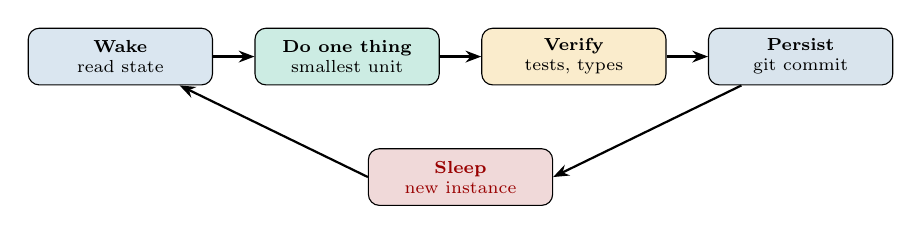
\begin{tikzpicture}[
    box/.style={draw, rounded corners=4pt, minimum width=2.6cm,
                minimum height=0.8cm, font=\scriptsize, align=center},
    arr/.style={-{Stealth[length=2mm]}, thick},
    scale=0.9, transform shape
]
    \node[box, fill=softblue!20]   (wake)  at (0,0)      {\textbf{Wake}\\read state};
    \node[box, fill=softgreen!20]  (work)  at (3.2,0)    {\textbf{Do one thing}\\smallest unit};
    \node[box, fill=softorange!20] (check) at (6.4,0)    {\textbf{Verify}\\tests, types};
    \node[box, fill=level1!50] (commit)at (9.6,0)    {\textbf{Persist}\\git commit};
    \node[box, fill=harvardcrimson!15, text=harvardcrimson] (sleep) at (4.8,-1.7) {\textbf{Sleep}\\new instance};

    \draw[arr] (wake)   -- (work);
    \draw[arr] (work)   -- (check);
    \draw[arr] (check)  -- (commit);
    \draw[arr] (commit) -- (sleep.east);
    \draw[arr] (sleep.west) -- (wake);
\end{tikzpicture}
\end{center}

\vspace{0.2em}
\begin{columns}[T]
\column{0.55\textwidth}
\textbf{Why it works.} Each iteration starts with a \emph{fresh, clean} context
window. Memory between runs lives only on disk: \texttt{git log},
\texttt{progress.txt}, a JSON task list. No drift, no sycophancy, no
``I forgot what we were doing.''

\column{0.43\textwidth}
\begin{alertblock}{When NOT to use it}
\scriptsize
Open-ended research, anything without an automatic verifier (tests, types,
benchmark passes/fails). Without a hard \emphc{stop condition}, the loop
will spin forever.
\end{alertblock}
\end{columns}
\end{frame}

% --- Ralph Loop (official plugin) ---
\begin{frame}[fragile]{The \texttt{/ralph-loop} Plugin (Anthropic-verified)}
\small
The simplest implementation: a \texttt{Stop} hook that re-injects the original
prompt every time Claude finishes, until a \emph{completion promise string}
appears in the output.

\vspace{0.3em}
\begin{columns}[T]
\column{0.50\textwidth}
\textbf{Install \& launch:}
\begin{lstlisting}[style=bash, basicstyle=\scriptsize\ttfamily]
# Inside Claude Code
/plugin marketplace add ralph-loop
/plugin install ralph-loop

# Run an autonomous loop
/ralph-loop "Implement
   passing pytest tests in
   tests/test_estimator.py.
   Stop when all green."
   --max-iterations 10
   --completion-promise "DONE"

# Cancel anytime
/cancel-ralph
\end{lstlisting}

\column{0.48\textwidth}
\textbf{What it gives you:}
\begin{itemize}\itemsep0pt
    \item Iteration counter, hard cap
    \item Files \& git history preserved across iterations
    \item Loop exits on \texttt{DONE} or budget
    \item One-line cancel
\end{itemize}

\vspace{0.3em}
\begin{block}{Best-practice prompts}
\scriptsize
\begin{itemize}\itemsep0pt
    \item Make the \emphc{completion promise} machine-checkable
        (``output \texttt{ALL\_TESTS\_PASS}'' beats ``done when you think it's good'').
    \item Pin a \emph{verifier}: \texttt{pytest -q}, \texttt{ruff}, \texttt{mypy --strict}.
    \item Set a small \texttt{--max-iterations} (5--10); raise only after one clean run.
\end{itemize}
\end{block}
\end{columns}
\end{frame}

% --- snarktank ralph (PRD-driven) ---
\begin{frame}[fragile]{\texttt{snarktank/ralph}: PRD-Driven Multi-Story Loops}
\scriptsize
For projects too large for a single prompt, the community \texttt{ralph.sh} script
(Ghuntley et al., 2025) runs Claude Code (or Amp) on a list of stories from a
PRD, one per iteration, until every story has \texttt{passes: true}.

\vspace{0.3em}
\begin{columns}[T]
\column{0.50\textwidth}
\textbf{Setup:}
\begin{lstlisting}[style=bash, basicstyle=\tiny\ttfamily]
# Add the marketplace inside Claude Code
/plugin marketplace add snarktank/ralph
/plugin install ralph-skills@ralph-marketplace

# 1. Generate a PRD via the prd skill
> Load the prd skill and create a PRD
  for: "DiD estimator with cluster-robust SE,
  unit tests, and a Markdown report".

# 2. Convert PRD -> JSON via the ralph skill
> Load the ralph skill and convert
  tasks/prd-did.md to prd.json.

# 3. Launch the loop (15 iter cap)
./scripts/ralph/ralph.sh --tool claude 15
\end{lstlisting}

\column{0.48\textwidth}
\textbf{Inside each iteration:}
\begin{enumerate}\itemsep0pt
  \item Pick the highest-priority story with \texttt{passes:false}
  \item Implement it (one story only)
  \item Run quality checks (\texttt{pytest}, \texttt{mypy}, \texttt{ruff})
  \item Commit if checks pass
  \item Mark the story \texttt{passes:true} in \texttt{prd.json}
  \item Append learnings to \texttt{progress.txt}
  \item \emph{Sleep, spawn fresh Claude.}
\end{enumerate}

\vspace{0.3em}
\begin{block}{Memory between iterations}
\tiny
Only three things survive: \emphc{git history} (all prior commits),
\emphc{prd.json} (which stories are done), and \emphc{progress.txt}
(append-only learnings). Everything else is wiped — by design.
\end{block}
\end{columns}
\end{frame}

% --- Ralph guardrails for econ research ---
\begin{frame}{Ralph Loops for Economics Research: Guardrails}
\scriptsize
Closed-loop autonomy is powerful and dangerous in equal measure. A short rule
set keeps it research-grade.

\vspace{0.3em}
\begin{columns}[T]
\column{0.50\textwidth}
\textbf{Hard prerequisites}
\begin{enumerate}\itemsep0pt
  \item \emphc{Verifier or no loop.} If you can't write a script that returns
        ``pass/fail,'' don't run a Ralph loop on it.
  \item \emphc{Tight stories.} ``Add cluster-robust SE to \texttt{estimate.py}''
        --- yes. ``Replicate Acemoglu (2001)'' --- no.
  \item \emphc{Cost cap.} \texttt{--max-iterations} \emph{and} per-iteration
        \texttt{timeout 600}.
  \item \emphc{Hooks on.} \texttt{PreToolUse} guards on \texttt{data/raw/};
        \texttt{Stop} auto-commit.
  \item \emphc{Git branch.} Always run on a throw-away feature branch.
\end{enumerate}

\column{0.48\textwidth}
\begin{alertblock}{Two failure modes to expect}
\tiny
\textbf{Compounding errors.} A wrong type-stub in iteration~3 propagates to
iterations 4--15. Mitigation: short loops, frequent diff review.

\vspace{0.3em}
\textbf{Token blow-up.} At \$0.50/iter, a 100-iter Opus loop is \$50.
Watch \texttt{/cost}.
\end{alertblock}

\vspace{0.2em}
\textbf{Closed loops change the question.} You stop asking
``how do I get Claude to do this?'' and start asking ``what is the smallest
machine-checkable spec that makes this loop terminate?''
\end{columns}

\vspace{0.2em}
\textbf{Hands-on:} \emphc{Exercise 12} --- a 5-iteration Ralph loop on a tiny estimator with \texttt{pytest} as verifier.
\end{frame}

% ============================================================================
% PART VIII: FROM DATA TO PAPER & REPLICATION  (15 min)
% ============================================================================

\begin{frame}{}
\vfill
\begin{center}
{\Huge \textcolor{uzhblue}{\textbf{Part VIII}}}\\[12pt]
{\LARGE From Raw Data to a Paper Section\\[4pt]
\& AI Agents for Paper Replication}\\[6pt]
{\small 15 minutes (includes Exercise 7)}
\end{center}
\vfill
\end{frame}

% --- Mincer mini-demo: prompt ---
\begin{frame}[fragile]{Warm-Up Demo: Mincer Wage Equation~\livedemo}
\scriptsize
A 30-second demo: one prompt, one publication-ready table, one figure.
Level 3 applied to the simplest regression in labor economics.

\vspace{0.2em}
\textbf{The Mincer equation} (Mincer, 1974):
$\log(\text{wage}) = \beta_0 + \beta_1\,\text{educ} + \beta_2\,\text{exper} + \beta_3\,\text{exper}^2 + \beta_4\,\text{female} + \varepsilon$

{\scriptsize $\beta_1 \approx 0.08$: each extra year of schooling raises wages by $\sim$8\%. The $\text{exper}^2$ term captures the concavity of lifecycle earnings. Every labor economist knows the expected answer, making this a perfect verifiable demo.}

\vspace{0.2em}
\begin{columns}[T]
\column{0.52\textwidth}
\textbf{The prompt (copy--paste):}
\begin{lstlisting}[style=prompt, basicstyle=\tiny\ttfamily, frame=single]
> Role: applied labor economist.
  Data: wage1 from the `wooldridge` package.
  Model:
    log(wage) = b0 + b1*educ + b2*exper
              + b3*exper^2 + b4*female + u
  Outputs:
  1) outputs/mincer_table.tex -- booktabs,
     SE in parentheses, stars .01/.05/.10.
  2) outputs/mincer_figure.pdf -- scatter
     of educ vs log(wage) + fitted partial
     line; serif font, 6x4 inches.
  Constraints: do NOT modify raw data.
  Verify: print summary and assert
         0.07 < b1 < 0.10.
\end{lstlisting}

\column{0.44\textwidth}
\textbf{What this prompt ships (all 6 components):}
\begin{itemize}\itemsep0pt
  \item \textbf{Role} --- applied labor economist
  \item \textbf{Context} --- data source named
  \item \textbf{Task} --- equation specified
  \item \textbf{Constraints} --- no raw modification
  \item \textbf{Output} --- exact paths \& formats
  \item \textbf{Verification} --- coefficient range
\end{itemize}

\vspace{0.2em}
\emphc{Runnable reference:}~\selfstudy~\texttt{lectures/lecture\_06\_B17\_agentic\_programming/code/mincer\_demo.py}
reproduces this output locally in \textasciitilde{}3~seconds. Self-study readers:
\texttt{python3 mincer\_demo.py} now, then look at the next slide for the artifacts.
\end{columns}
\end{frame}

% --- Mincer mini-demo: output ---
\begin{frame}{\selfstudy~~Mincer Demo: What Claude Produces}
\scriptsize
After \textasciitilde{}45 seconds Claude writes the script, runs it, and emits
the two artifacts below (actual outputs of \texttt{lectures/lecture\_06\_B17\_agentic\_programming/code/mincer\_demo.py}).

\vspace{0.2em}
\begin{columns}[T]
\column{0.52\textwidth}
\textbf{\texttt{outputs/mincer\_table.tex}:}

\vspace{0.3em}
\centering
\renewcommand{\arraystretch}{1.15}
\begin{tabular}{lcc}
\toprule
Variable & Coefficient & Std. Error \\
\midrule
Constant             & \phantom{-}0.3905$^{***}$  & (0.1022) \\
Education (years)    & \phantom{-}0.0841$^{***}$  & (0.0070) \\
Experience (years)   & \phantom{-}0.0389$^{***}$  & (0.0048) \\
Experience$^2$       &          $-$0.0007$^{***}$ & (0.0001) \\
Female               &          $-$0.3372$^{***}$ & (0.0363) \\
\midrule
$R^2$                & \multicolumn{2}{c}{0.3996} \\
Observations         & \multicolumn{2}{c}{526}    \\
\bottomrule
\end{tabular}

\vspace{0.3em}
\raggedright
\scriptsize \emph{Notes:} OLS on \texttt{wage1} (CPS 1976). \texttt{***} $p<0.01$.

\column{0.44\textwidth}
\textbf{\texttt{outputs/mincer\_figure.pdf}:}

\vspace{0.2em}
\centering
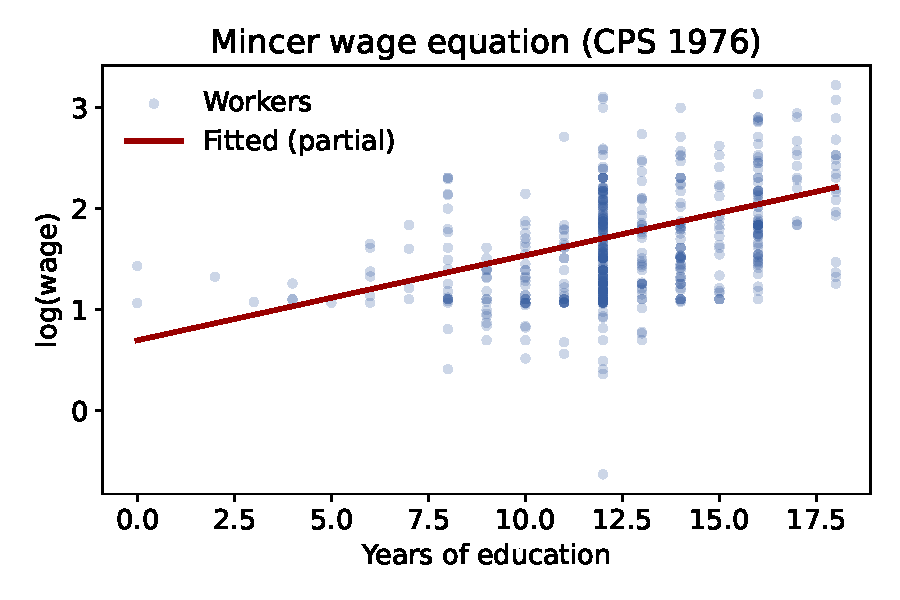
\includegraphics[width=\linewidth]{../code/outputs/mincer_figure.pdf}

\vspace{0.2em}
\raggedright
\scriptsize
Scatter of education vs $\log(\text{wage})$ with fitted partial line
(\texttt{exper}, \texttt{female} held at means).
\end{columns}

\vspace{0.3em}
\begin{exampleblock}{Takeaway}
\scriptsize
A single Level-3 prompt $\to$ reproducible code $\to$ LaTeX-ready table $+$
PDF figure, saved to the right paths, with a verification assertion. This is
the unit we will compose into the full pipeline.
\end{exampleblock}
\end{frame}

% --- Pipeline ---
\begin{frame}[fragile]{The Full Research Pipeline}
\begin{columns}[T]
\column{0.35\textwidth}
\begin{center}
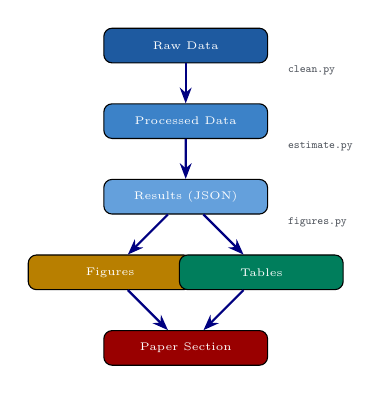
\begin{tikzpicture}[
    arr/.style={-{Stealth[length=2mm]}, thick, uzhblue},
    script/.style={font=\tiny\ttfamily, text=uzhgreydark, anchor=west},
    scale=0.8, transform shape
]
    \node[pipestep=level5] (raw) at (0,5) {Raw Data};
    \node[script] at (1.5,4.6) {clean.py};
    \node[pipestep=level4] (proc) at (0,3.8) {Processed Data};
    \node[script] at (1.5,3.4) {estimate.py};
    \node[pipestep=level3] (res) at (0,2.6) {Results (JSON)};
    \node[script] at (1.5,2.2) {figures.py};
    \node[pipestep=softorange!80!black] (fig) at (-1.2,1.4) {Figures};
    \node[pipestep=softgreen!80!black] (tab) at (1.2,1.4) {Tables};
    \node[pipestep=harvardcrimson] (paper) at (0,0.2) {Paper Section};

    \draw[arr] (raw) -- (proc);
    \draw[arr] (proc) -- (res);
    \draw[arr] (res) -- (fig);
    \draw[arr] (res) -- (tab);
    \draw[arr] (fig) -- (paper);
    \draw[arr] (tab) -- (paper);
\end{tikzpicture}
\end{center}

\column{0.62\textwidth}
\textbf{Goal:} A pipeline where \texttt{python run\_all.py} reproduces the entire paper from scratch.

\vspace{0.3em}
\textbf{Six prompts, one per step:}
\begin{enumerate}\itemsep1pt
    \item[\textbf{1.}] \textbf{Data diagnostics}---shape, missingness, outliers\\
    {\scriptsize ``Read data/raw/panel.csv. Do NOT modify it. Write report.''}
    \item[\textbf{2.}] \textbf{Cleaning}---thresholds in \texttt{config.py}\\
    {\scriptsize ``Based on the report, write code/clean.py. Use pathlib.''}
    \item[\textbf{3.}] \textbf{Estimation}---specs in code, results to JSON\\
    {\scriptsize ``Estimate using pyfixest: Y $\sim$ D $|$ firm+year, cluster(firm).''}
    \item[\textbf{4.}] \textbf{Figures}---publication-ready PDFs\\
    {\scriptsize ``Event study plot, serif font, 7$\times$4, 300 DPI.''}
    \item[\textbf{5.}] \textbf{Tables}---raw LaTeX with \texttt{booktabs}\\
    {\scriptsize ``SEs in parentheses. Stars: * $<$0.1, ** $<$0.05, *** $<$0.01.''}
    \item[\textbf{6.}] \textbf{Paper draft}---using notation from CLAUDE.md\\
    {\scriptsize ``400--600 words, RES style. Use $\backslash$citet\{\} and $\backslash$citep\{\}.''}
\end{enumerate}

\vspace{0.2em}
{\scriptsize Then: ``Write \texttt{run\_all.py} that chains all steps with \texttt{--dry-run}.''}
\end{columns}
\end{frame}

% --- Replication ---
\begin{frame}[fragile]{AI Agents for Paper Replication}
\begin{columns}[T]
\column{0.48\textwidth}
\textbf{Why replication is the best exercise:}
\begin{itemize}\itemsep2pt
    \item Bounded task with a \emphc{clear success criterion} (do the numbers match?)
    \item Forcing function for all skills above
    \item Genuine research contribution
    \item Standard starting point for extending methods
\end{itemize}

\vspace{0.3em}
\textbf{The Replication Ladder:}

\vspace{0.2em}
\scriptsize
\renewcommand{\arraystretch}{1.1}
\begin{tabular}{p{3.5cm} l}
\toprule
\textbf{Paper Type} & \textbf{AI Success} \\
\midrule
Well-documented + code & \textcolor{darkgreen}{\textbf{High}} \\
Well-documented, no code & \textcolor{darkgreen}{\textbf{High}} \\
Sparse docs, standard method & \textcolor{softorange}{\textbf{Moderate}} \\
Novel method, first paper & \textcolor{softorange}{\textbf{Low--Mod}} \\
Outside training data & \textcolor{darkred}{\textbf{Low}} \\
\bottomrule
\end{tabular}

\column{0.48\textwidth}
\textbf{The replication prompt:}
\begin{lstlisting}[style=prompt, basicstyle=\tiny\ttfamily]
> Role: Replication engineer.
  Paper: [title, authors, DOI]
  Mission: Replicate ALL figures+tables.
  Hard rules:
  1. CANNOT use authors' code
  2. Track in notes/todo.md
  3. Commit after each step
  4. If stuck x3, write blocked.md, STOP
  Before implementing:
  - Extract figure axes, ranges, CIs
  - Write plan to notes/plan.md
  Implementation: Python + NumPy/SciPy
  Figures to figures/replication/ (PDF)
  Final: "Paper value vs. Our value"
\end{lstlisting}

\vspace{0.2em}
\textbf{Verification:}\\
{\scriptsize For each result: paper value vs.\ your value.\\
$<5\%$ error = \checkmark match; 5--20\% = $\sim$ close; $>20\%$ = \ding{55} fail.}
\end{columns}
\end{frame}

% --- Exercises 6 & 7 ---
\begin{frame}[fragile]{Exercises 6 \& 7 {\small(25 + 10 min)}}
\begin{columns}[T]
\column{0.48\textwidth}
\begin{exampleblock}{Ex.\,6: Data $\to$ Figures $\to$ LaTeX (25 min)}
\small
Use \texttt{lectures/lecture\_06\_B17\_agentic\_programming/code/generate\_synthetic\_data.py} to create data, then build a mini pipeline:
\begin{enumerate}\itemsep0pt
    \item Run data diagnostics (use your \texttt{/data-diagnostics} skill!)
    \item Estimate DiD: $\log(\text{revenue}) \sim \text{treated} \times \text{post}$
    \item Generate an event study plot
    \item Generate a LaTeX table
    \item Verify: true effect = 0.05, estimate should be close
\end{enumerate}

{\scriptsize Stretch: wire into \texttt{run\_all.py}}
\end{exampleblock}

\column{0.48\textwidth}
\begin{exampleblock}{Ex.\,7: Replicate a Method (10 min)}
\small
Choose a target:
\begin{itemize}\itemsep0pt
    \item \textbf{Beginner:} Lasso forecasting\\[-2pt]
    {\scriptsize Stock \& Watson (2012), Figure 1}
    \item \textbf{Intermediate:} SINDy\\[-2pt]
    {\scriptsize Brunton et al.\ (2016), Figure 3}
    \item \textbf{Advanced:} DEQN policy function\\[-2pt]
    {\scriptsize From earlier-lecture notebooks}
\end{itemize}

\vspace{0.2em}
Use the replication prompt. Start with figure analysis before implementation.
\end{exampleblock}
\end{columns}
\end{frame}

% ============================================================================
% PART IX: VERIFICATION, ETHICS & BEST PRACTICES  (15 min)
% ============================================================================

\begin{frame}{}
\vfill
\begin{center}
{\Huge \textcolor{uzhblue}{\textbf{Part IX}}}\\[12pt]
{\LARGE Verification, Ethics \& Best Practices}\\[6pt]
{\small 15 minutes}
\end{center}
\vfill
\end{frame}

% --- Verification ---
\begin{frame}[fragile]{The Cardinal Rule: Never Skip Verification}
\small
\begin{alertblock}{The Invisible Failure Mode}
AI code that \emphc{crashes} is visible. AI code that runs cleanly but clusters standard errors at the wrong level is \emphc{invisible}. This is worse than a bug.
\end{alertblock}

\vspace{0.2em}
\begin{columns}[T]
\column{0.48\textwidth}
\textbf{Mandatory verification steps:}
\begin{enumerate}\itemsep2pt
    \item \textbf{Synthetic data test:}\\
    {\scriptsize Generate data where true effect = 0.5. Run estimator. Coefficient should be $\approx$0.5.}
    \item \textbf{Reproduce a known result:}\\
    {\scriptsize Run on data with published answers.}
    \item \textbf{Check identification in code:}\\
    {\scriptsize Print first stage, plot residuals.}
    \item \textbf{Simple-case regression:}\\
    {\scriptsize Does it reduce to OLS when it should?}
\end{enumerate}

\column{0.48\textwidth}
\textbf{Five things AI gets wrong in econometrics:}
\begin{enumerate}\itemsep1pt
    \item \textbf{SE clustering}---wrong level or omitted
    \item \textbf{FE in nonlinear models}---wrong incidental parameters correction
    \item \textbf{Identification}---estimates any model, even misspecified
    \item \textbf{Panel structure}---forgets \texttt{sort\_values(['id','t'])}
    \item \textbf{Merge logic}---inner/outer/left confusion
\end{enumerate}

\vspace{0.2em}
{\scriptsize For each: the fix is a \emphc{constraint in your prompt}. Add the check explicitly.}
\end{columns}
\end{frame}

% --- Ethics: journal disclosure norms ---
\begin{frame}{Disclosure Norms by Publisher (2023--2026)}
\scriptsize
Norms have moved fast. Check the \emph{specific} journal's instructions before submission.

\vspace{0.2em}
\renewcommand{\arraystretch}{1.05}
\begin{tabular}{p{2.5cm} p{1.4cm} p{7.5cm}}
\toprule
\textbf{Publisher} & \textbf{Author?} & \textbf{Required disclosure} \\
\midrule
ICMJE (medical) & \textcolor{darkred}{No} & List in Methods + Acknowledgements; humans accountable \\
\textit{Nature} & \textcolor{darkred}{No} & Document use in Methods \\
\textit{Science} & \textcolor{darkred}{No} & Permission \emph{ex ante}; cover letter + Acknowledgements \\
Elsevier & \textcolor{darkred}{No} & Statement at end of manuscript; no AI-generated images \\
Springer Nature & \textcolor{darkred}{No} & Methods + Acknowledgements; no AI images \\
AEA (\textit{AER}/\textit{JEL}/\textit{P\&P}) & \textcolor{darkred}{No} & Disclose \emph{substantive} use; replication package must be deterministic \\
QJE / RES / JPE & \textcolor{darkred}{No} & Disclose substantive use; check current guidelines \\
COPE (industry std.) & \textcolor{darkred}{No} & ``LLMs cannot meet authorship criteria'' (2023) \\
\bottomrule
\end{tabular}

\vspace{0.3em}
\begin{alertblock}{Bottom line for PhD students}
\tiny
Treat \emphc{any} substantive LLM use (text, code, analysis, ideation) as disclosable until proven otherwise. Disclose model name, version, date in Methods; keep a prompt log next to the replication package.
\end{alertblock}
\end{frame}

% --- Replication packages under AI ---
\begin{frame}[fragile]{Replication Packages in the Age of LLMs}
\scriptsize
\begin{columns}[T]
\column{0.55\textwidth}
\textbf{The new failure mode.} An LLM call is \emph{non-deterministic}. Re-running an analysis no longer means identical numbers---unless you freeze the LLM output as code and check it in.

\vspace{0.2em}
\textbf{AEA Data Editor (Vilhuber et al.\ 2020--24) requires:}
\begin{enumerate}\itemsep0pt
    \item Pipeline artifacts re-runnable \emph{without} re-querying any LLM
    \item Data lineage (raw $\to$ processed $\to$ tables) fully scripted
    \item Random seeds pinned and documented
\end{enumerate}

\vspace{0.2em}
\textbf{What to ship:}
\begin{itemize}\itemsep0pt
    \item All code, including LLM-generated code as \emphc{frozen} files
    \item Conda / uv lockfile + Docker image where feasible
    \item \texttt{prompts.md} with model + version + date per artifact
    \item \texttt{CLAUDE.md} (sensitive-path rules redacted)
\end{itemize}

\column{0.43\textwidth}
\begin{block}{Anti-patterns}
\tiny
\begin{itemize}\itemsep0pt
    \item ``Re-run \texttt{claude} on \texttt{prompt.md}.'' \emph{Will not reproduce.}
    \item Calling an LLM inside \texttt{run\_all.py} without seed/version pin.
    \item Ralph commit messages as documentation.
    \item Pushing \texttt{.claude/audit.log} or \texttt{.env} to a public repo.
\end{itemize}
\end{block}

\vspace{0.2em}
\textbf{Preventing hallucinated citations:}
\begin{lstlisting}[style=prompt, basicstyle=\tiny\ttfamily]
> Do NOT invent citations.
  Only cite refs in
  references.bib. If unsure:
  [CITE: author, year -- verify]
\end{lstlisting}
{\tiny Walters \& Wilder (2023): 47--69\%\ hallucination rate. Real fix: \emph{retrieval} (Zotero MCP, Semantic Scholar), not instruction.}
\end{columns}
\end{frame}

% --- Privacy: GDPR, EU AI Act, Swiss FADP ---
\begin{frame}{Data Privacy: GDPR, the EU AI Act, and Swiss FADP}
\small
This is a course in Switzerland with EU/EEA data flows. The legal frame
matters when you point Claude at thesis/RA datasets.

\vspace{0.3em}
\begin{columns}[T]
\column{0.50\textwidth}
\textbf{Three regimes that apply:}
\begin{itemize}\itemsep1pt
    \item \emphc{GDPR} (EU 2016/679): personal data leaves the EU when sent to Anthropic's US-hosted API. Needs \emph{either} Standard Contractual Clauses, an Adequacy Decision, or specific consent. Article~9 ``special categories'' (health, ethnicity, political views) is more restrictive.
    \item \emphc{Swiss FADP} (revised 2023): equivalent regime; same SCC mechanism via the Swiss Federal Data Protection and Information Commissioner.
    \item \emphc{EU AI Act} (in force 2024--2026): general-purpose models are regulated; \emph{research exemption} under Art.~2 covers academic research, but transparency obligations remain.
\end{itemize}

\column{0.48\textwidth}
\textbf{Practical defaults for empirical research:}
\begin{itemize}\itemsep0pt
    \item[\textcolor{darkred}{\ding{55}}] Raw IRB / PII / Article-9 data: never to the API
    \item[\textcolor{darkred}{\ding{55}}] API keys, tokens, credentials: never
    \item[\textcolor{softorange}{\textbf{?}}] DUA-protected data: re-read the agreement before using a Claude session
    \item[\textcolor{darkgreen}{\checkmark}] Hash / synthesize / aggregate first; send the derivative
    \item[\textcolor{darkgreen}{\checkmark}] Use the \texttt{PreToolUse} hook + \texttt{CLAUDE.md} read-only paths
    \item[\textcolor{darkgreen}{\checkmark}] Document the data class (public, internal, restricted) in \texttt{CLAUDE.md}
\end{itemize}

\vspace{0.3em}
{\tiny Anthropic Zero-Data-Retention agreements exist for enterprise use;
ask your university IT before relying on them for sensitive flows.}
\end{columns}
\end{frame}

% --- Boris tip 10 ---
\begin{frame}{One More: Output Styles for Auditable Workflows}
\small
\boristip{10} Enable the ``Explanatory'' output style in \texttt{/config} to
have Claude explain the \emph{why} behind its changes. Great for learning
and for auditing AI-written code that ends up in your replication package.

\vspace{0.4em}
\begin{block}{A workflow that satisfies all three regimes}
\small
\begin{enumerate}\itemsep1pt
    \item \texttt{CLAUDE.md} declares data classes and read-only paths.
    \item \texttt{PreToolUse} hook hard-blocks \texttt{data/raw/}, \texttt{.env}, etc.
    \item \texttt{PostToolUse} audit-log captures \emph{file paths only}
        (not Bash commands; secrets stay out of \texttt{.claude/audit.log}).
    \item Every LLM-generated artifact is checked into git as a \emph{file},
        not a re-runnable prompt.
    \item \texttt{prompts.md} ships with the replication package: model name,
        version, date for every artifact.
    \item Co-authors review the diff before merge --- AI is a junior contributor,
        not a co-author.
\end{enumerate}
\end{block}
\end{frame}

% --- Boris Tips Summary ---
\begin{frame}{Boris Cherny's 10 Claude Code Tips (Summary)}
\scriptsize
Boris Cherny created Claude Code at Anthropic. These tips come from his team's daily workflow.

\vspace{0.3em}
\renewcommand{\arraystretch}{1.15}
\begin{tabular}{c p{4cm} p{7cm}}
\toprule
\textbf{\#} & \textbf{Tip} & \textbf{Key Detail} \\
\midrule
1 & Do more in \emphc{parallel} & 3--5 worktrees, each with its own Claude session \\
2 & Start complex tasks in \emphc{Plan Mode} & Pour energy into the plan so Claude one-shots implementation \\
3 & Invest in your \emphc{CLAUDE.md} & ``Update CLAUDE.md so you don't make that mistake again'' \\
4 & Create custom \emphc{skills} & If you do it $>$1$\times$/day, make it a slash command \\
5 & Claude fixes most \emphc{bugs} by itself & Paste error + ``fix.'' Don't micromanage how. \\
6 & Level up your \emphc{prompting} & Challenge Claude; write detailed specs; reduce ambiguity \\
7 & \emphc{Terminal} setup matters & Ghostty, statusline, color-coded tabs, voice dictation \\
8 & Use \emphc{subagents} & Offload research to keep main context clean \\
9 & Use Claude for \emphc{data/analytics} & Connect to databases via CLI or MCP \\
10 & \emphc{Learning} with Claude & Enable Explanatory output; generate visual explanations \\
\bottomrule
\end{tabular}

\vspace{0.3em}
{\scriptsize Source: Boris Cherny (creator of Claude Code), 2025.}
\end{frame}

% --- Self-Study Extensions ---
\begin{frame}{Self-Study Extensions: Exercises 0, 8--12}
\small
The 75-minute classroom slot covers Exercises 1--7. The companion file
\texttt{exercise\_prompts.md} ships with five extension exercises you can do
on your own time:

\vspace{0.4em}
\renewcommand{\arraystretch}{1.2}
\begin{tabular}{c p{4.5cm} p{6cm}}
\toprule
\textbf{Ex.} & \textbf{Topic} & \textbf{Time / focus} \\
\midrule
0  & ``Hello Claude'' & 10 min --- first contact, zero setup \\
8  & Mincer wage regression demo & 20--30 min --- end-to-end OLS pipeline \\
9  & Specialist subagents (econ, MC, backtest) & 30--45 min --- per-agent practice \\
10 & Hooks: audit log + path guard + strategic-revision skill & 45--60 min \\
11 & Subagent-driven Monte Carlo design & 30--45 min --- design \& critique \\
\textbf{12} & \textbf{Ralph autonomous loop} (Part VII) & 30--45 min --- closed-loop run on a tiny estimator \\
\bottomrule
\end{tabular}

\vspace{0.4em}
{\scriptsize Solutions sketches in \texttt{exercise\_solutions.md}; consult only
\emph{after} attempting each exercise.}
\end{frame}

% ============================================================================
% WRAP-UP & REFERENCES
% ============================================================================

\begin{frame}{}
\vfill
\begin{center}
{\Huge \textcolor{uzhblue}{\textbf{Wrap-Up}}}\\[12pt]
{\LARGE Quick Reference \& Key Takeaways}
\end{center}
\vfill
\end{frame}

% --- Quick Reference ---
\begin{frame}{Quick Reference Card {\small(print this)}}
\small
\begin{columns}[T]
\column{0.32\textwidth}
\textbf{\textcolor{uzhblue}{Before Every Session}}
\begin{itemize}\itemsep0pt
    \item[\scriptsize$\square$] \texttt{git commit} checkpoint
    \item[\scriptsize$\square$] Update CLAUDE.md status
\end{itemize}

\vspace{0.2em}
\textbf{\textcolor{uzhblue}{Context Hygiene}}
\begin{itemize}\itemsep0pt
    \item[\scriptsize$\square$] \texttt{/compact} at $\sim$20 turns
    \item[\scriptsize$\square$] Write to \texttt{progress.md}
    \item[\scriptsize$\square$] Fresh session per sub-task
    \item[\scriptsize$\square$] Use subagents for research
\end{itemize}

\column{0.34\textwidth}
\textbf{\textcolor{uzhblue}{Prompt Checklist (Level 3)}}
\begin{itemize}\itemsep0pt
    \item[\scriptsize$\square$] Role or context set?
    \item[\scriptsize$\square$] File names and paths?
    \item[\scriptsize$\square$] Constraints (NOT to do)?
    \item[\scriptsize$\square$] Output format specified?
    \item[\scriptsize$\square$] Verification step?
\end{itemize}

\vspace{0.2em}
\textbf{\textcolor{uzhblue}{Key Commands}}\\
{\scriptsize\ttfamily
/compact, /clear, /cost, /init\\
Ctrl+C, ESC, Shift+Tab (plan)}

\column{0.30\textwidth}
\textbf{\textcolor{uzhblue}{Safety}}
\begin{itemize}\itemsep0pt
    \item[\scriptsize$\square$] No IRB/PII data
    \item[\scriptsize$\square$] \texttt{.claudeignore} active
    \item[\scriptsize$\square$] Review diff before commit
    \item[\scriptsize$\square$] Interrupt early
\end{itemize}

\vspace{0.2em}
\textbf{\textcolor{uzhblue}{After Every Session}}
\begin{itemize}\itemsep0pt
    \item[\scriptsize$\square$] \texttt{git diff HEAD}
    \item[\scriptsize$\square$] \texttt{git add -p \&\& commit}
    \item[\scriptsize$\square$] Update \texttt{progress.md}
    \item[\scriptsize$\square$] Update CLAUDE.md
\end{itemize}
\end{columns}
\end{frame}

% --- Key Takeaways ---
\begin{frame}{Key Takeaways}
\scriptsize
\begin{enumerate}\itemsep1pt
    \item \textbf{The bottleneck has shifted} from coding to \emphc{specification}. Your domain expertise is the competitive advantage.
    \item \textbf{Explore $\to$ Plan $\to$ Implement $\to$ Commit.} Pour energy into the plan; let Claude one-shot the implementation.
    \item \textbf{Level 3 prompts} (specific + context + constraints + output + verify) are the single highest-impact skill.
    \item \textbf{CLAUDE.md + skills + subagents + hooks} = the infrastructure for safe, scalable, reproducible agentic workflows.
    \item \textbf{Closed loops change the question} from ``how do I get Claude to do this?'' to ``what is the smallest machine-checkable spec that makes this loop terminate?'' (Ralph).
    \item \textbf{Never skip verification.} Synthetic data with known answers; check SE clustering; verify every citation.
    \item \textbf{Cost is a research input.} Track \texttt{/cost}; pick the cheapest model that keeps quality; cap every loop.
    \item \textbf{Reproducibility under AI is non-trivial.} LLM calls are non-deterministic: freeze artifacts as code, pin model+version+date.
    \item \textbf{AI is a fast second-year PhD student.} Excellent at known methods; mediocre at novel ones. Your judgment on identification, specification, and interpretation remains essential.
\end{enumerate}
\end{frame}

% --- Discussion ---
\begin{frame}{Discussion Questions}
\begin{enumerate}\itemsep6pt
    \item \textbf{The ``black box'' problem:} If Claude wrote the code, do you truly understand your results?

    \item \textbf{Competitive dynamics:} If AI reduces the cost of empirical execution, what changes in the market for research ideas?

    \item \textbf{Refereeing:} What signals should you look for as a referee to assess robustness of AI-generated results?

    \item \textbf{Graduate training:} Should PhD programs still require students to write estimation code by hand?

    \item \textbf{Level 5 autonomy:} Under what conditions would you let an agent run a full analysis unsupervised for two hours?
\end{enumerate}
\end{frame}

% --- Readings ---
\begin{frame}{Readings \& Resources}
\tiny
\textbf{AI for economists:}
\begin{itemize}\itemsep0pt
    \item Korinek (2023). ``Generative AI for Economic Research.'' \emph{JEL} 61(4): 1281--1317.
    \item Korinek \& Balwit (2023). ``Aligned AI as a Tool for Economists.'' \emph{AEA P\&P} 113: 348--53.
    \item Schluntz \& Zhang (2024). ``Building Effective Agents.'' Anthropic engineering blog.
\end{itemize}

\textbf{Empirical evidence on AI productivity:}
\begin{itemize}\itemsep0pt
    \item METR (Model Evaluation \& Threat Research, 2025). Early-2025 AI \& experienced OSS (open-source software) developer productivity --- found a 19\% \emph{slow-down}.
    \item Cui, Demirer, Jaffe, et al.\ (2024). Generative AI in high-skilled work (Microsoft/MIT field experiment).
    \item Brynjolfsson, Li, Raymond (2025). ``Generative AI at Work.'' \emph{QJE} (call-center RCT).
    \item Peng, Kalliamvakou, et al.\ (2023). Copilot RCT on developer productivity.
    \item Walters \& Wilder (2023). Fabricated citations from ChatGPT. \emph{Sci.\ Rep.}\ 13: 14045.
    \item Liu, Lin, et al.\ (2024). ``Lost in the Middle.'' \emph{TACL} 12: 157--173.
\end{itemize}

\textbf{Practitioner / Claude Code:}
\begin{itemize}\itemsep0pt
    \item Cherny (2025). ``10 Claude Code Tips from the Creator of Claude Code.''
    \item Goldsmith-Pinkham (2026). ``Getting Started with Claude Code.'' \emph{paulgp.substack.com}.
    \item Bilionis et al.\ (2026). ``We Asked an AI Agent to Replicate Three Papers.'' \emph{ebilionis.substack.com}.
    \item Ghuntley et al.\ (2025). \texttt{snarktank/ralph} --- PRD-driven autonomous loop.
\end{itemize}

\textbf{Tools:}
Claude Code \url{https://docs.claude.com/en/docs/claude-code} \,$\bullet$\,
Anthropic Academy \url{https://www.anthropic.com/learn} \,$\bullet$\,
MCP \url{https://modelcontextprotocol.io} \,$\bullet$\,
Ralph Loop \url{https://claude.com/plugins/ralph-loop} \,$\bullet$\,
\texttt{snarktank/ralph} \url{https://github.com/snarktank/ralph}

\vspace{0.1em}
Course repo: \url{https://github.com/sischei/Deep_Learning_for_Solving_And_Estimating_Dynamic_Economic_Models}.
\end{frame}

% --- Where to Next ---
\begin{frame}{Where to Next: PINNs \& Continuous-Time HA Models}
\small
\begin{columns}[T]
\column{0.55\textwidth}
\textbf{What we built today.} A research workflow:
\begin{itemize}\itemsep0pt
    \item Claude Code with \texttt{CLAUDE.md}, skills, subagents, hooks
    \item Plan~$\to$~Implement~$\to$~Verify discipline
    \item \emphc{Closed loops} via Ralph for spec-driven autonomy
\end{itemize}

\vspace{0.4em}
\textbf{Tomorrow we apply it.} Day~6 introduces:
\begin{itemize}\itemsep0pt
    \item \emphc{Physics-Informed Neural Networks} (PINNs) for HJB equations
    \item Continuous-time \emphc{heterogeneous-agent} models
    \item Two reference notebook stacks (PINNs~$\times$~5; CT~HA~$\times$~3)
\end{itemize}

\column{0.43\textwidth}
\begin{block}{Suggested workflow for the next lecture}
\scriptsize
For every notebook you read:
\begin{enumerate}\itemsep0pt
  \item Drop it into a Claude Code session.
  \item \texttt{> Explain the residual loss / KFE on lines~X--Y.}
  \item Use the \emphc{verifier} subagent on any equation you change.
  \item For nontrivial extensions, draft a 5-story PRD and run Ralph
        (Part~VII) with \texttt{pytest} on a synthetic ground-truth case.
\end{enumerate}
\end{block}

\vspace{0.3em}
{\scriptsize The \emphc{Day-2--4 recap}: from DEQNs to autodiff, sequence space, OLG.
Day~6 swaps PDEs for the Bellman residual; the workflow stays the same.}
\end{columns}
\end{frame}

\end{document}
